This chapter presents the results of the proposed approaches implementation. Additional details of the models are given and their performance for training and testing data. 

\section{Variables Selection}
\label{s:results_data_selection}

The Pearson correlation is calculated to select the optimal input variables for the system. \autoref{t:correlation_table} summarizes the correlation values for the three target variables where \ac{COD}\textsubscript{D}, \ac{COD}\textsubscript{EQ}, and \ac{MLVSS} are one-day a head shifted variables.

%\begin{longtable}{@{}l *{2}{rr}}
\begin{longtable}[h!]{@{}l *{2}{rr}}
\caption[Portrait Table, short caption]{Variables Correlation}
\label{t:correlation_table}
\\
%   
\toprule%


 {\bfseries Variable} & {\bfseries COD\textsubscript{D} } & {\bfseries COD\textsubscript{EQ}} & {\bfseries MLVSS}
\\

\cmidrule[0.4pt](r{0.125em}){1-1}%
\cmidrule[0.4pt](lr{0.125em}){2-4}%
%\cmidrule[0.4pt](lr{0.125em}){4-5}%
%\cmidrule[0.4pt](lr{0.125em}){5-6}%


  \endfirsthead

\endhead

        Flow\_to\_EQ & 0.14 & -0.14 & -0.025  \\ 
        BT\_C\_MLSS & 0.11 & -0.43 & 0.88  \\ 
        BT\_C\_MLVSS & 0.10 & -0.45 & 0.9  \\ 
        BT\_N\_MLSS & 0.10 & -0.44 & 0.88  \\ 
        BT\_N\_MLVSS & 0.10 & -0.44 & 0.88  \\ 
        D\_SS & 0.3 & 0.59 & -0.46  \\ 
        EQ\_N & 0.25 & 0.74 & -0.54  \\ 
        BT\_C\_N & 0.25 & 0.49 & -0.54  \\ 
        BT\_N\_N & 0.11 & 0.26 & -0.47  \\ 
        D\_N & 0.11 & 0.23 & -0.46  \\ 
        OxT\_pH & -0.12 & -0.33 & 0.27  \\ 
        EQ\_pH & -0.069 & 0.18 & -0.17  \\ 
        BT\_N\_pH & 0.057 & -0.045 & 0.083  \\ 
        D\_pH & 0.059 & -0.13 & 0.078  \\ 
        BT\_N\_DO & -0.1 & -0.37 & 0.14  \\ 
        BT\_C\_DO & -0.28 & -0.33 & 0.34  \\ 
        Clari\_DO & -0.17 & -0.43 & 0.27  \\ 
        ST\_COD & 0.22 & 0.63 & -0.44  \\ 
        D\_COD\_ON & 0.72 & 0.22 & 0.11  \\


\bottomrule

\end{longtable}

Variables that present a correlation higher than 0.2 are selected as inputs for the system. As a result, the input variables for each target variable are shown below:

\begin{itemize}
    \item \textbf{COD\textsubscript{D} :} D\_SS, BT\_C\_N, EQ\_N, BT\_C\_DO, ST\_COD, EQ\_COD, D\_COD\_ON.
    \item \textbf{COD\textsubscript{EQ} :} BT\_C\_MVLSS, D\_SS, EQ\_N, BT\_C\_N, OxT\_PH\_PM, BT\_N\_DO, Clari\_DO, ST\_COD, EQ\_COD.
    \item \textbf{MLVSS :} BT\_C\_MVLSS, D\_SS, EQ\_N, BT\_C\_N, OxT\_PH\_PM, BT\_C\_DO, Clari\_DO, ST\_COD, EQ\_COD.
\end{itemize}

It is necessary to standardize these variables to take them to similar level values. This step helps the model give the same level of relevance to each input variable no matter its magnitude value.

\begin{equation}
    X'_i = \frac{x_i - x_{mean}}{x_{std}}
\end{equation}

\begin{itemize}
    \item \begin{math}X'_i\end{math} is each standardized value.
    \item \begin{math}X_i\end{math} is each raw value.
    \item \begin{math}X_{mean}\end{math} is the mean value of the variable in the training dataset.
    \item \begin{math}X_{std}\end{math} is the standard deviation value of the variable in the training dataset.
\end{itemize}


\section{Approach 1}
\label{s:resutls-approach1}
The first approach conducts the time series decomposition just as described in \autoref{ss:time-series-decomposition} for each target variable. It estimates the trend and seasonal components by applying auto-regression of its past values, a process supported in the auto-correlation study just as mentioned in \autoref{ss:autocorrelation}. The residual component is predicted by a \ac{FFNN} that receives the inputs presented in \autoref{s:results_data_selection} and includes the real residual value as an additional input feature. The \ac{FFNN} architecture and the approach prediction results are presented below.
All model hyper-parameters were tuned by a grid search between the following options:

\begin{itemize}
    \item Loss = [mse, mae]
    \item Optimizer = [SGD, adam]
    \item Activation = [linear, tanh]
    \item Number of Layers = [1, 2]
    \item Number of Neurons per layer = [2, 4, 6, 8, 10, 12, 14, 16, 18, 20, 22, 24, 26, 28, 30, 32]
    \item Batch Normalization = [0, 1]
\end{itemize}

\subsection{COD Discharge}
\autoref{f:App1-codd-nn} shows the structure of the \ac{FFNN} used for \ac{COD}\textsubscript{D} residual prediction which hyper-parameters are presented below. \autoref{f:App1-codd} shows the prediction results of this approach where the orange line corresponds to model prediction over the training data, the red line to the model prediction over the testing samples. Finally, the blue one indicates the actual value the target variable takes.

\begin{figure}[h]
\centering
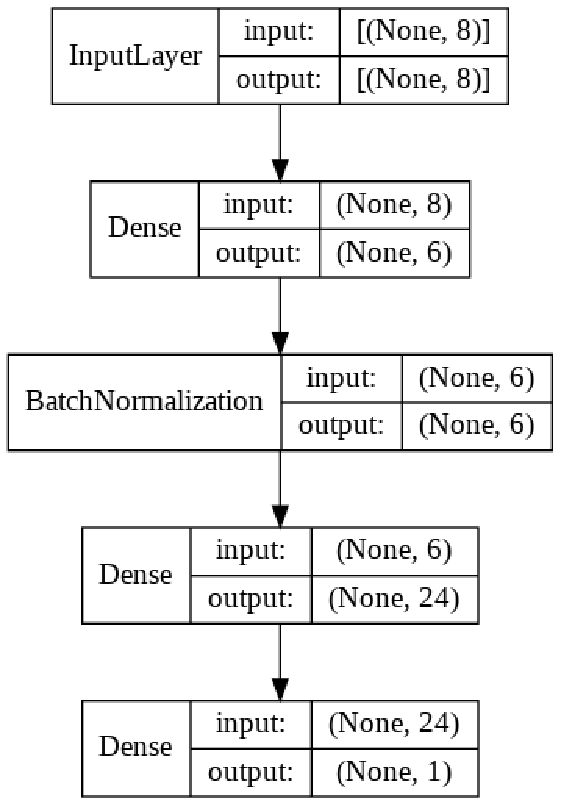
\includegraphics[width=0.4\linewidth]{figures/Ch5/App1_CODeq.pdf}
\caption{Approach 1 - COD\textsubscript{D} Network}
\label{f:App1-codd-nn}
\end{figure}

\begin{figure}[hb!]
\centering
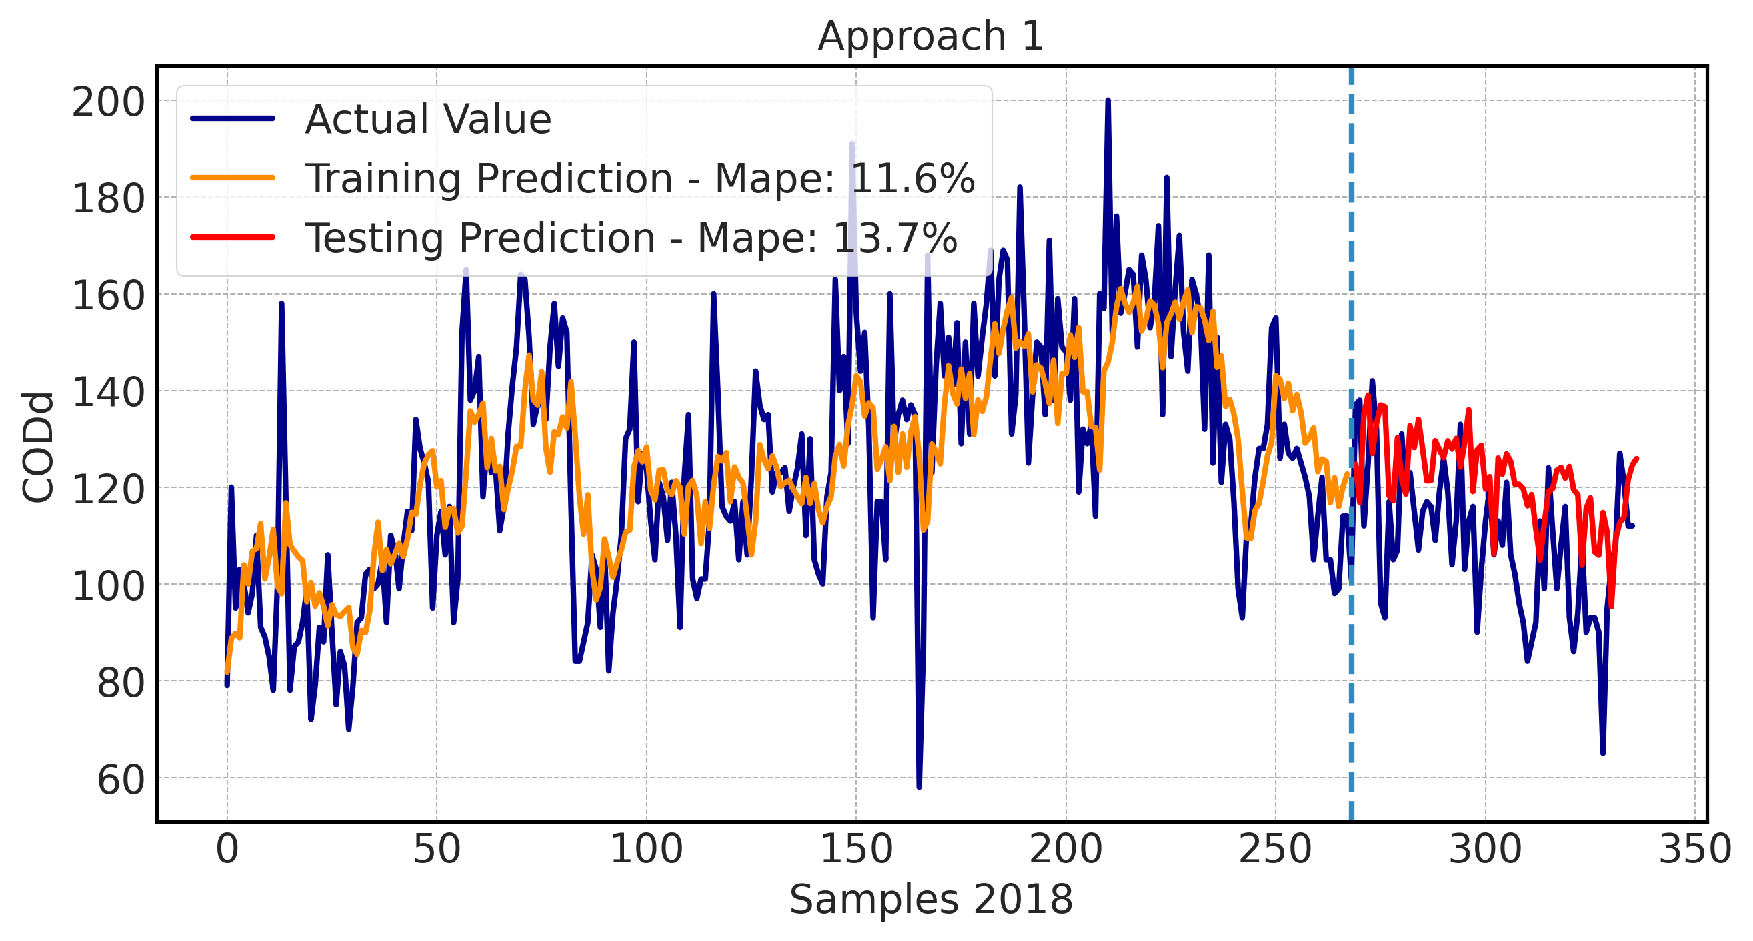
\includegraphics[width=\linewidth]{figures/Ch5/CODd-1.pdf}
\caption{Approach 1 - COD\textsubscript{D}}
\label{f:App1-codd}
\end{figure}

\begin{itemize}
    \item Loss = mse
    \item Optimizer = SGD
    \item Activation =  tanh
    \item Number of Layers = 2
    \item Number of Neurons per layer = [6, 24]
    \item Batch Normalization = 1
\end{itemize}

\subsection{COD Equalizer}
\autoref{f:App1-codeq-nn} shows the structure of the \ac{FFNN} used for \ac{COD}\textsubscript{EQ} residual prediction which hyper-parameters are presented below. \autoref{f:App1-codd} shows the prediction results of this approach.

\begin{itemize}
    \item Loss = mse
    \item Optimizer = SGD
    \item Activation =  Linear
    \item Number of Layers = 2
    \item Number of Neurons per layer = [10, 18]
    \item Batch Normalization = 1
\end{itemize}

\begin{figure}[h]
\centering
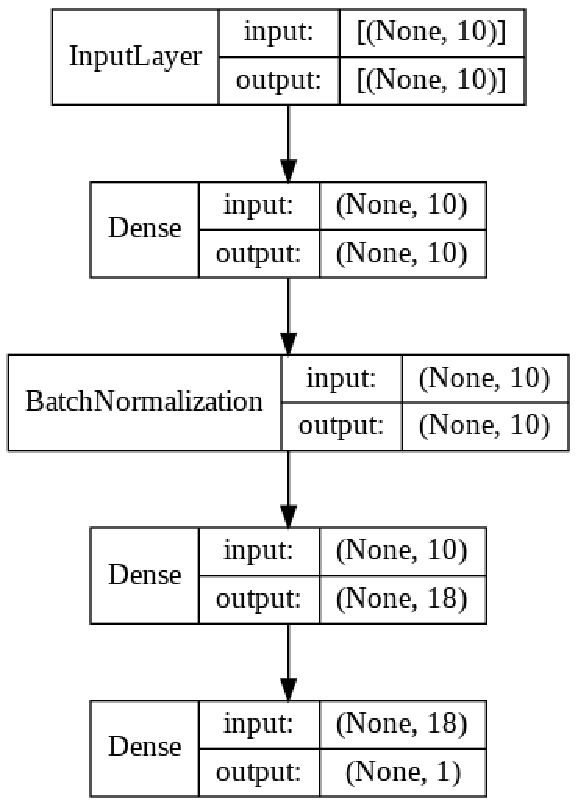
\includegraphics[width=0.4\linewidth]{figures/Ch5/App1_CODd.pdf}
\caption{Approach 1 - COD\textsubscript{EQ} Network}
\label{f:App1-codeq-nn}
\end{figure}

\begin{figure}[h]
\centering
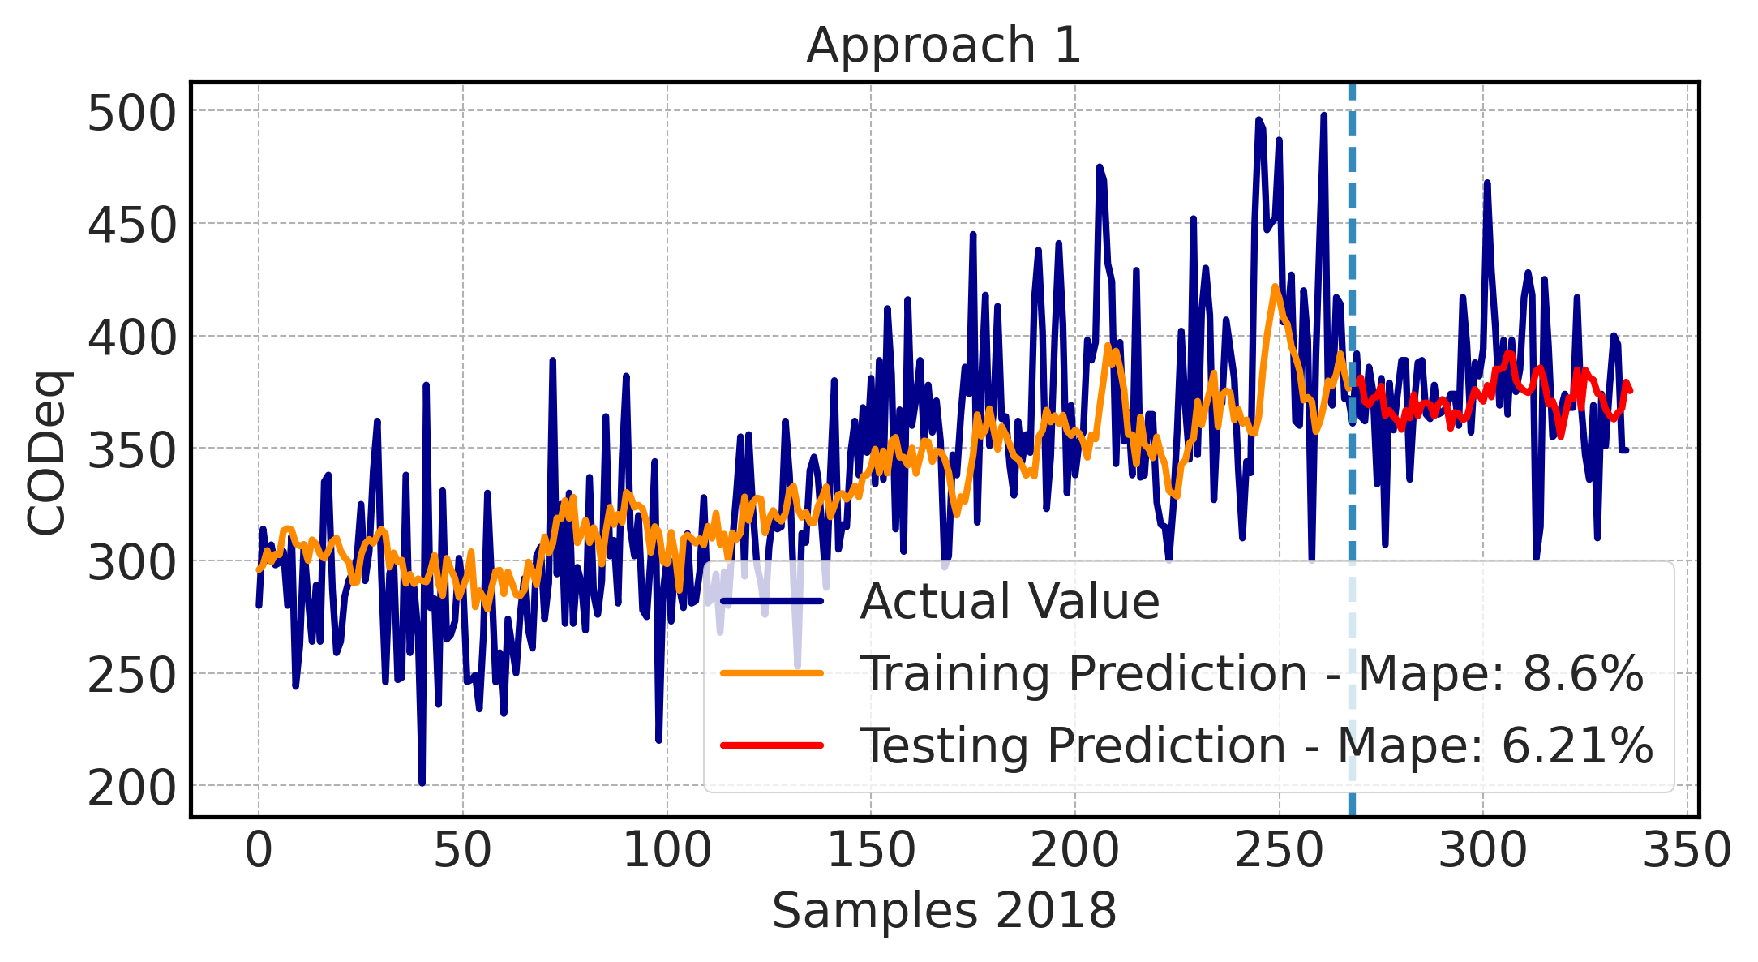
\includegraphics[width=\linewidth]{figures/Ch5/CODeq-1.pdf}
\caption{Approach 1 - COD\textsubscript{EQ}}
\label{f:App1-codeq}
\end{figure}

\subsection{MLVSS}

\autoref{f:App1-MLVSS-nn} shows the structure of the \ac{FFNN} used for \ac{MLVSS} residual prediction which hyper-parameters are presented below. \autoref{f:App1-MLVSS} shows the prediction results of this approach.

\begin{figure}[h!]
\centering
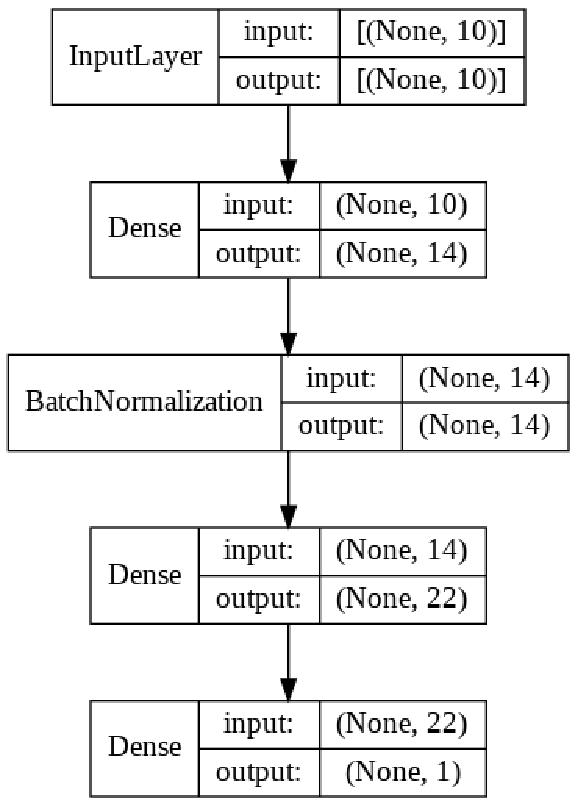
\includegraphics[width=0.4\linewidth]{figures/Ch5/App1_MLVSS.pdf}
\caption{Approach 1 - MLVSS Network}
\label{f:App1-MLVSS-nn}
\end{figure}

\begin{itemize}
    \item Loss = mse
    \item Optimizer = SGD
    \item Activation =  Relu
    \item Number of Layers = 2
    \item Number of Neurons per layer = [14, 22]
    \item Batch Normalization = 1
\end{itemize}
%------------------------------------------------
\begin{figure}[h]
\centering
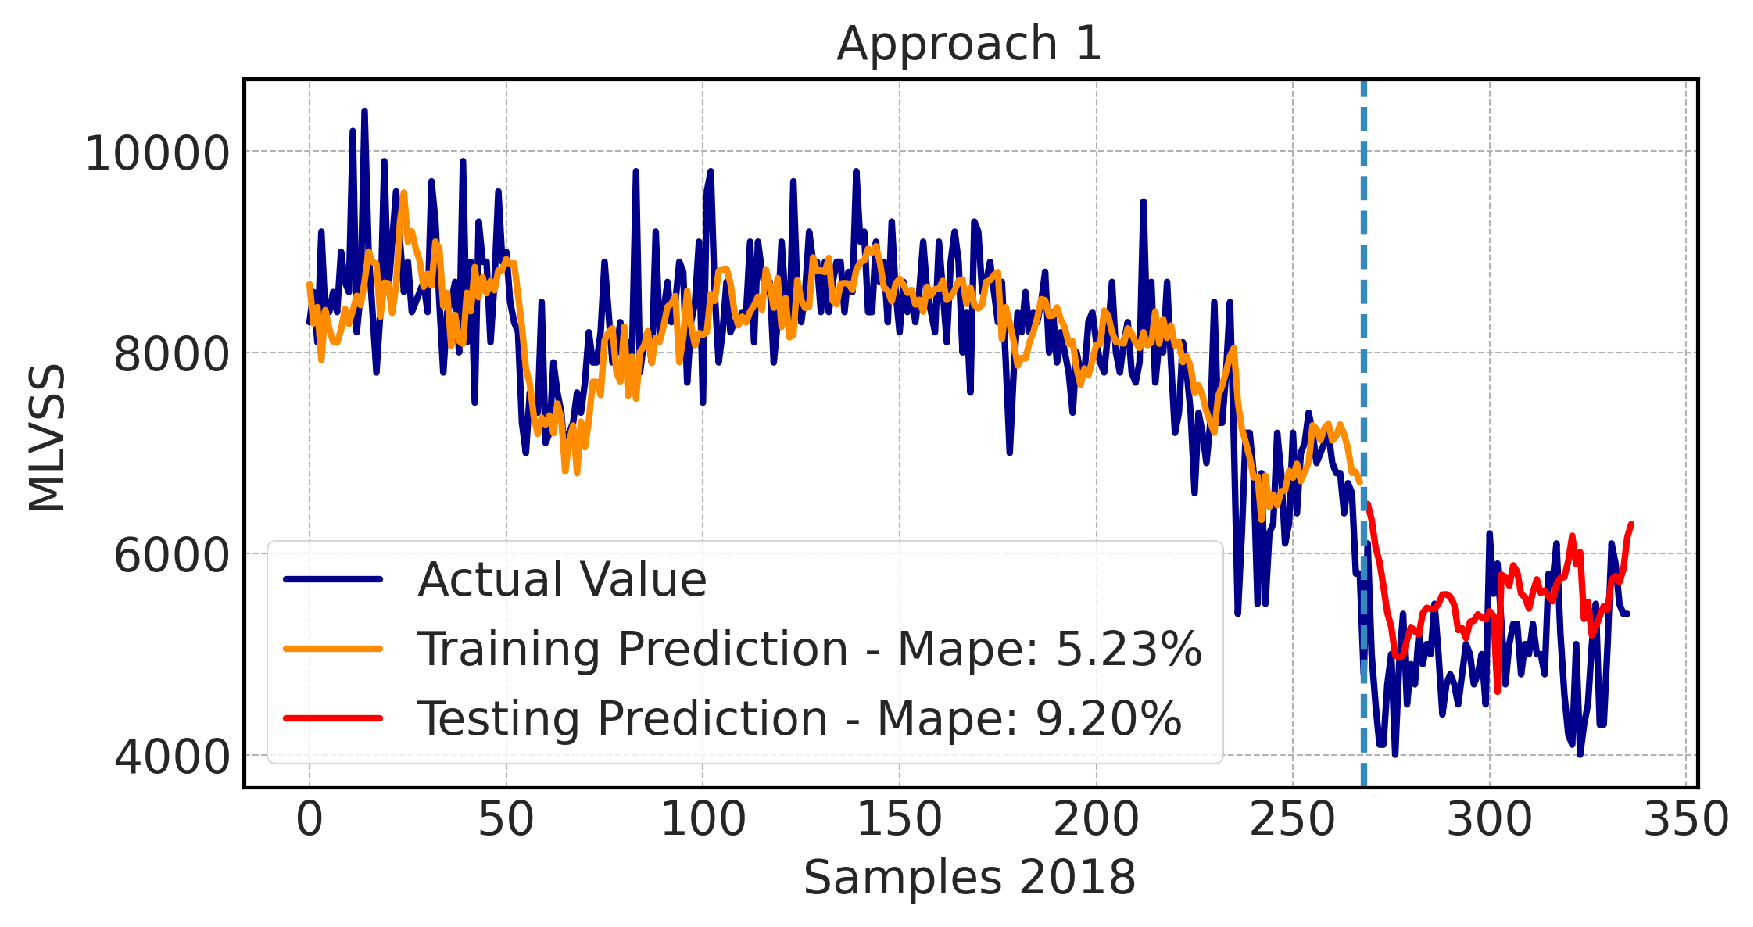
\includegraphics[width=\linewidth]{figures/Ch5/MLVSS-approach1.pdf}
\caption{Approach 1 - MLVSS}
\label{f:App1-MLVSS}
\end{figure}





\section{Approach 2}
The \ac{LSTM} architecture for each target variable and the approach prediction results are presented below. The \ac{LSTM} network implemented takes until seven past days to predict one day ahead.
All model hyper-parameters were tuned by a grid search within the following options:

\begin{itemize}
    \item Loss = [mse, mae]
    \item Optimizer = [SGD, adam]
    \item Activation = [Relu, linear, tanh]
    \item Number of Layers = [1, 2]
    \item Number of Neurons per layer = [2, 4, 6, 8, 10, 12, 14, 16, 18, 20, 22, 24, 26, 28, 30, 32]
    \item Batch Normalization = [0, 1]
    \item Dropout = [0, 1]
\end{itemize}

For Batch normalization and Dropout, zero means they are not included in the network.

\subsection{COD Discharge}
\autoref{f:App2-codd-nn} shows the structure of the \ac{LSTM} used for \ac{COD}\textsubscript{D} prediction which hyper-parameters are presented below. \autoref{f:App2-codd} shows the prediction results of this approach.

\begin{figure}[h]
\centering
 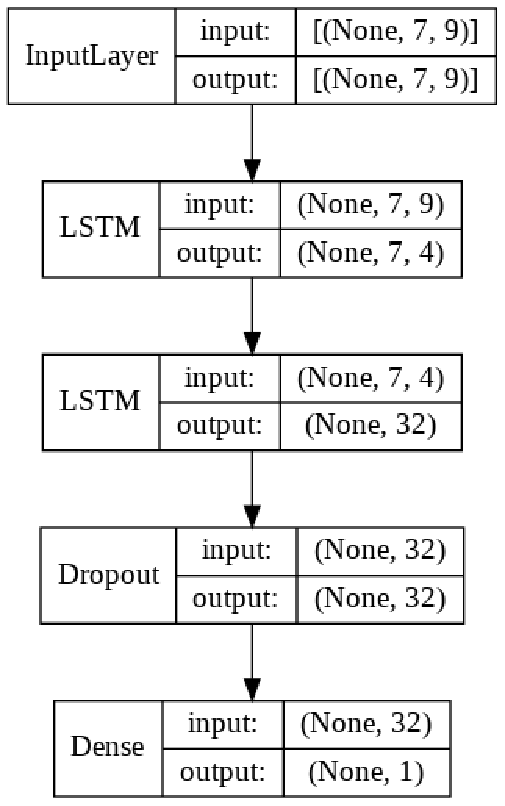
\includegraphics[width=0.4\linewidth]{figures/Ch5/App2_CODd.pdf}
\caption{Approach 2 - COD\textsubscript{D} LSTM Network}
\label{f:App2-codd-nn}
\end{figure}

\begin{figure}[h!]
\centering
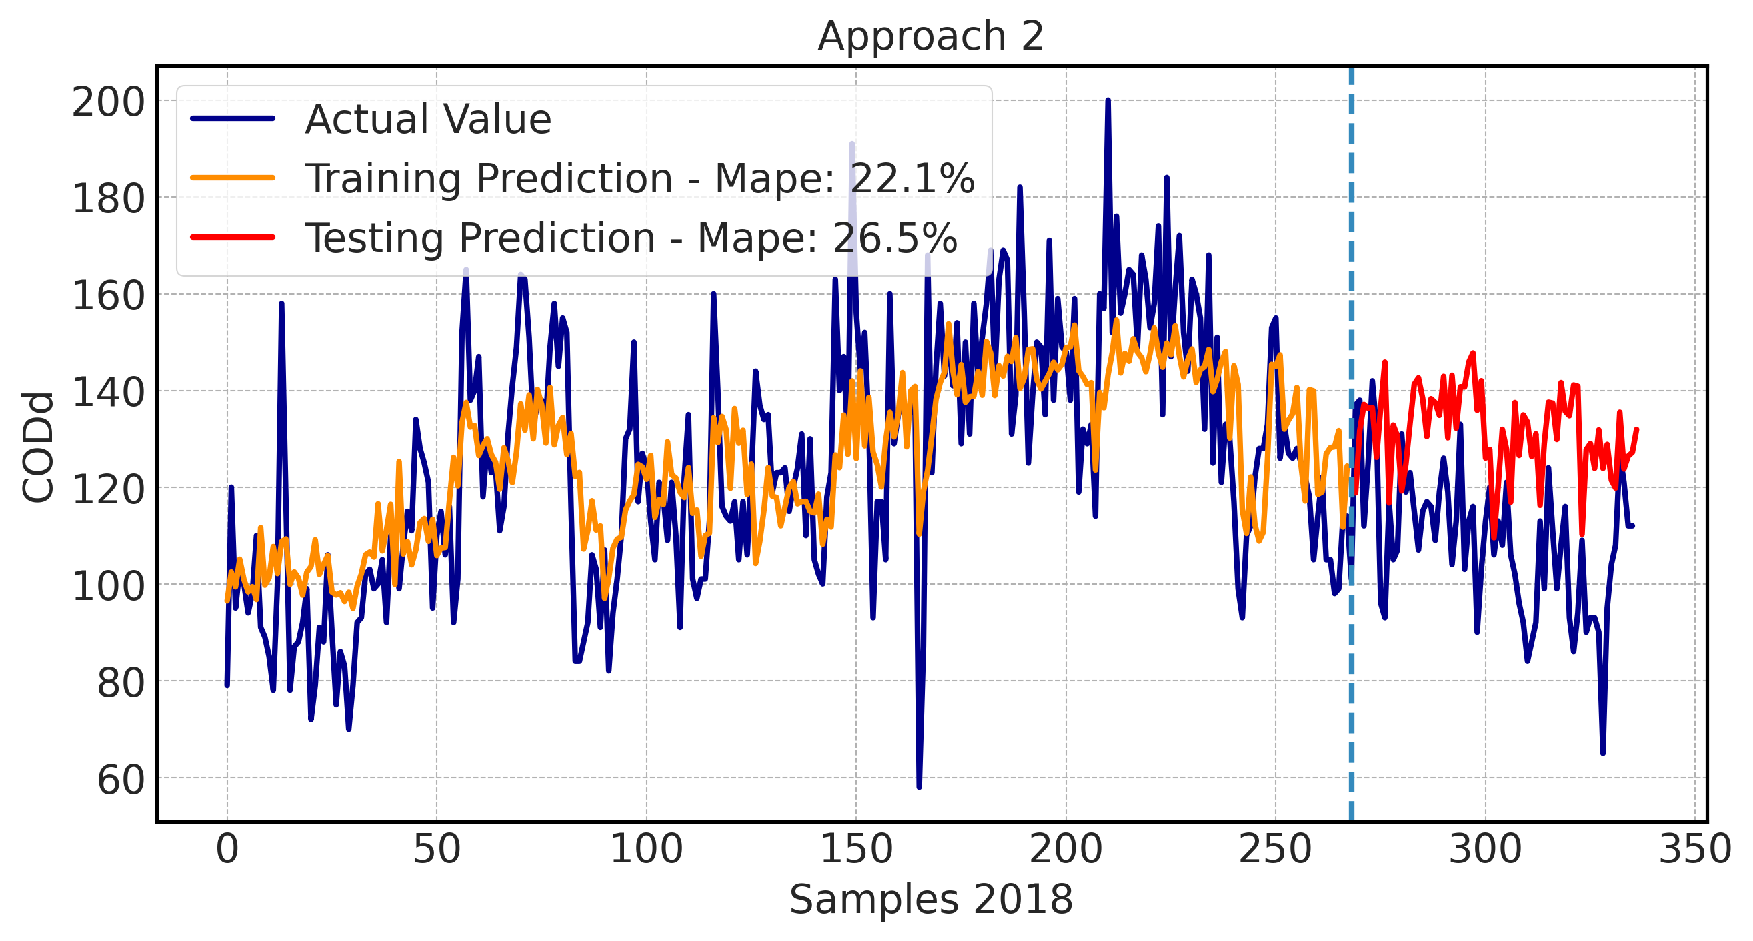
\includegraphics[width=\linewidth]{figures/Ch5/CODd-2.pdf}
\caption{Approach 2 - COD\textsubscript{D}}
\label{f:App2-codd}
\end{figure}

\begin{itemize}
    \item Loss = mse
    \item Optimizer = SGD
    \item Activation =  Tanh
    \item Number of Layers = 2
    \item Number of Neurons per layer = [4, 32]
    \item Batch Normalization = 0
    \item Dropout = 1
\end{itemize}

\subsection{COD Equalizer}
\autoref{f:App2-codeq-nn} shows the structure of the \ac{LSTM} used for \ac{COD}\textsubscript{EQ} prediction which hyper-parameters are presented below. \autoref{f:App2-codeq} shows the prediction results of this approach.

\begin{itemize}
    \item Loss = mse
    \item Optimizer = Adam
    \item Activation =  Tanh
    \item Number of Layers = 2
    \item Number of Neurons per layer = [2, 18]
    \item Batch Normalization = 1
    \item Dropout = 0
\end{itemize}

\begin{figure}[h]
\centering
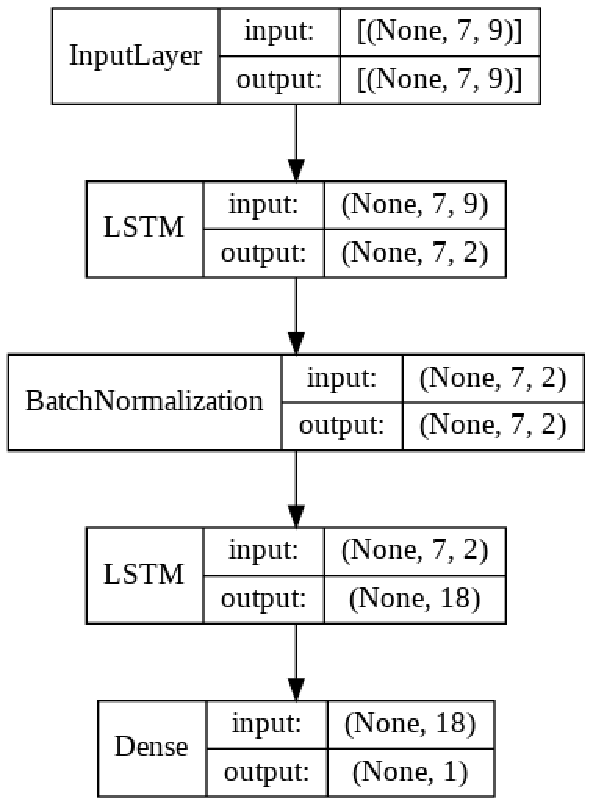
\includegraphics[width=0.4\linewidth]{figures/Ch5/App2_CODeq.pdf}
\caption{Approach 2 - COD\textsubscript{EQ} LSTM Network}
\label{f:App2-codeq-nn}
\end{figure}

\begin{figure}[h]
\centering
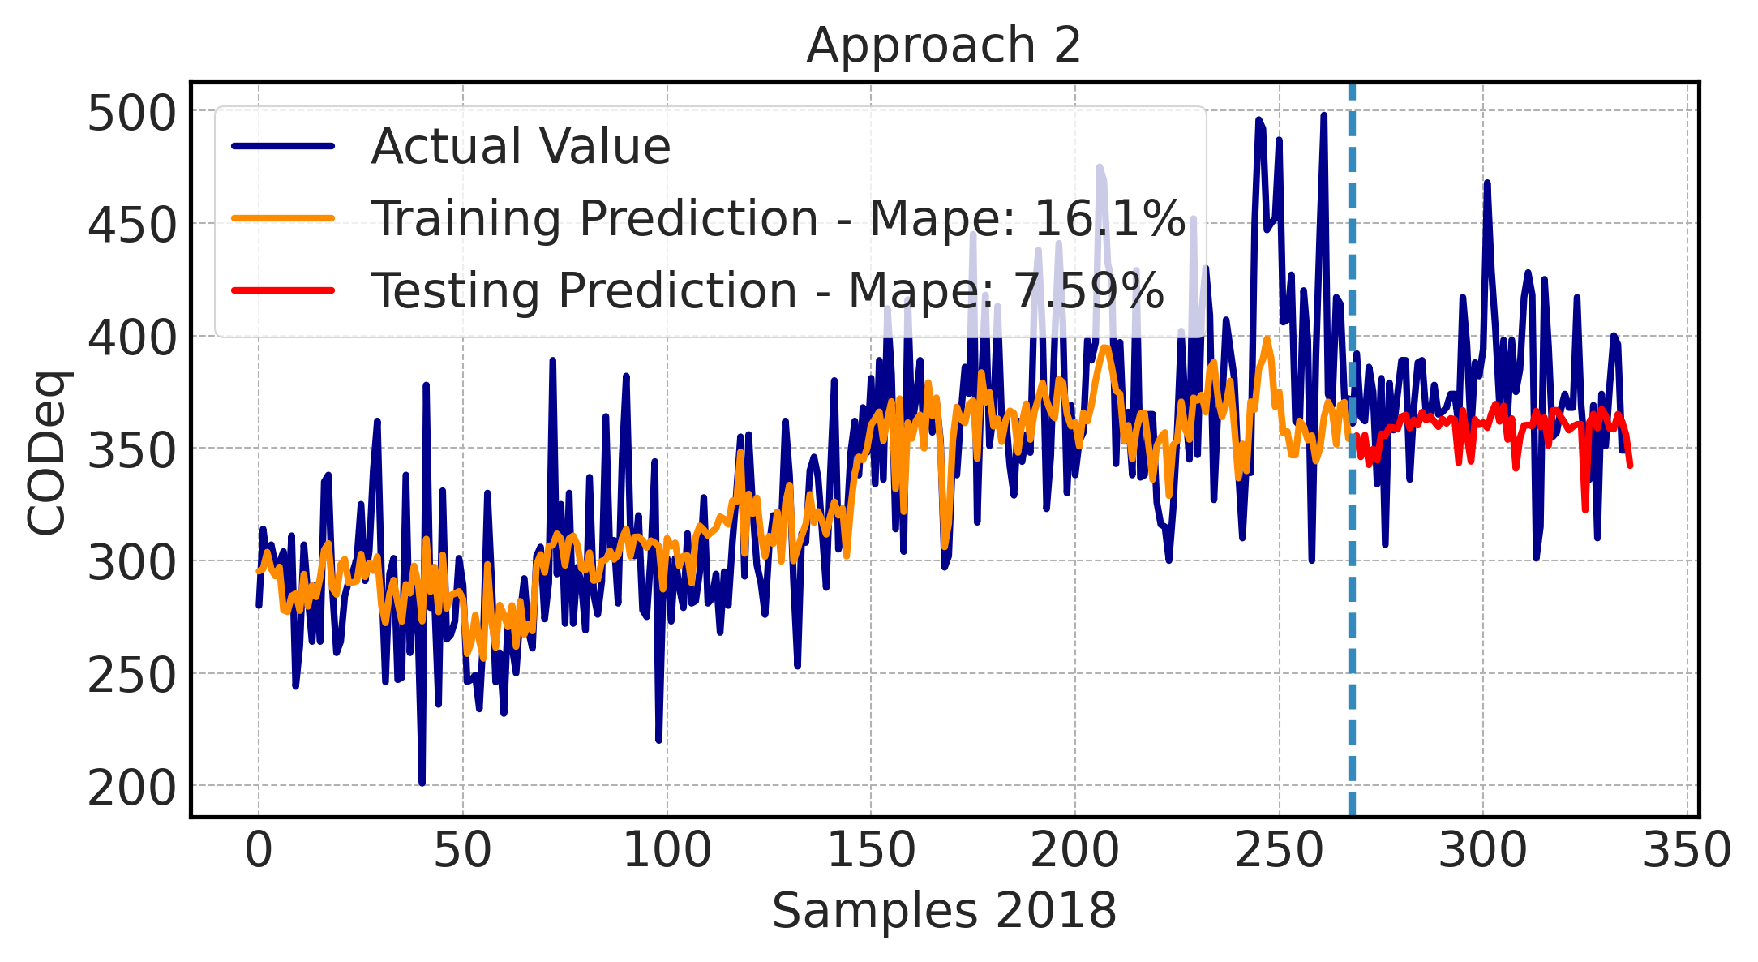
\includegraphics[width=\linewidth]{figures/Ch5/CODeq-2.pdf}
\caption{Approach 2 - COD\textsubscript{EQ}}
\label{f:App2-codeq}
\end{figure}

\subsection{MLVSS}
\autoref{f:App2-MLVSS-nn} shows the structure of the \ac{LSTM} used for \ac{MLVSS} prediction which hyper-parameters are presented below. \autoref{f:App2-MLVSS} shows the prediction results of this approach.

\begin{figure}[h]
\centering
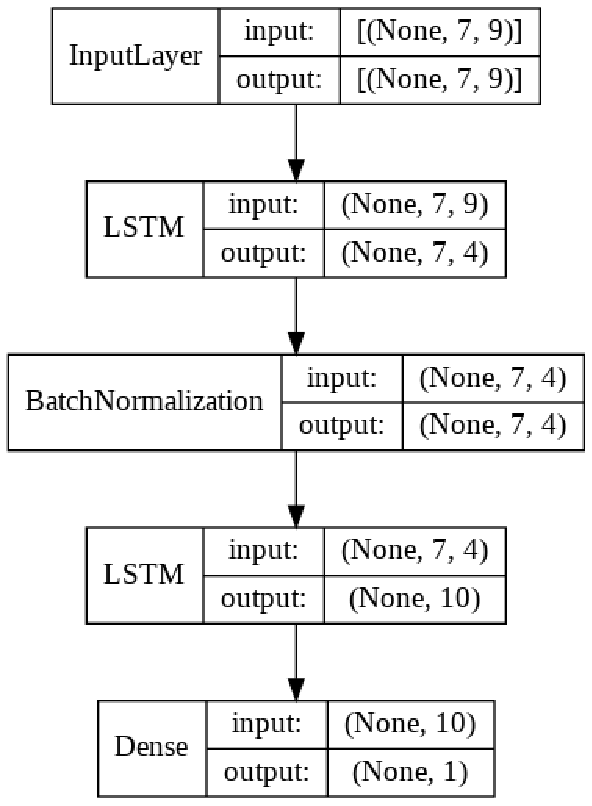
\includegraphics[width=0.4\linewidth]{figures/Ch5/App2_MLVSS.pdf}
\caption{Approach 2 - MLVSS LSTM Network}
\label{f:App2-MLVSS-nn}
\end{figure}

\begin{figure}[h]
\centering
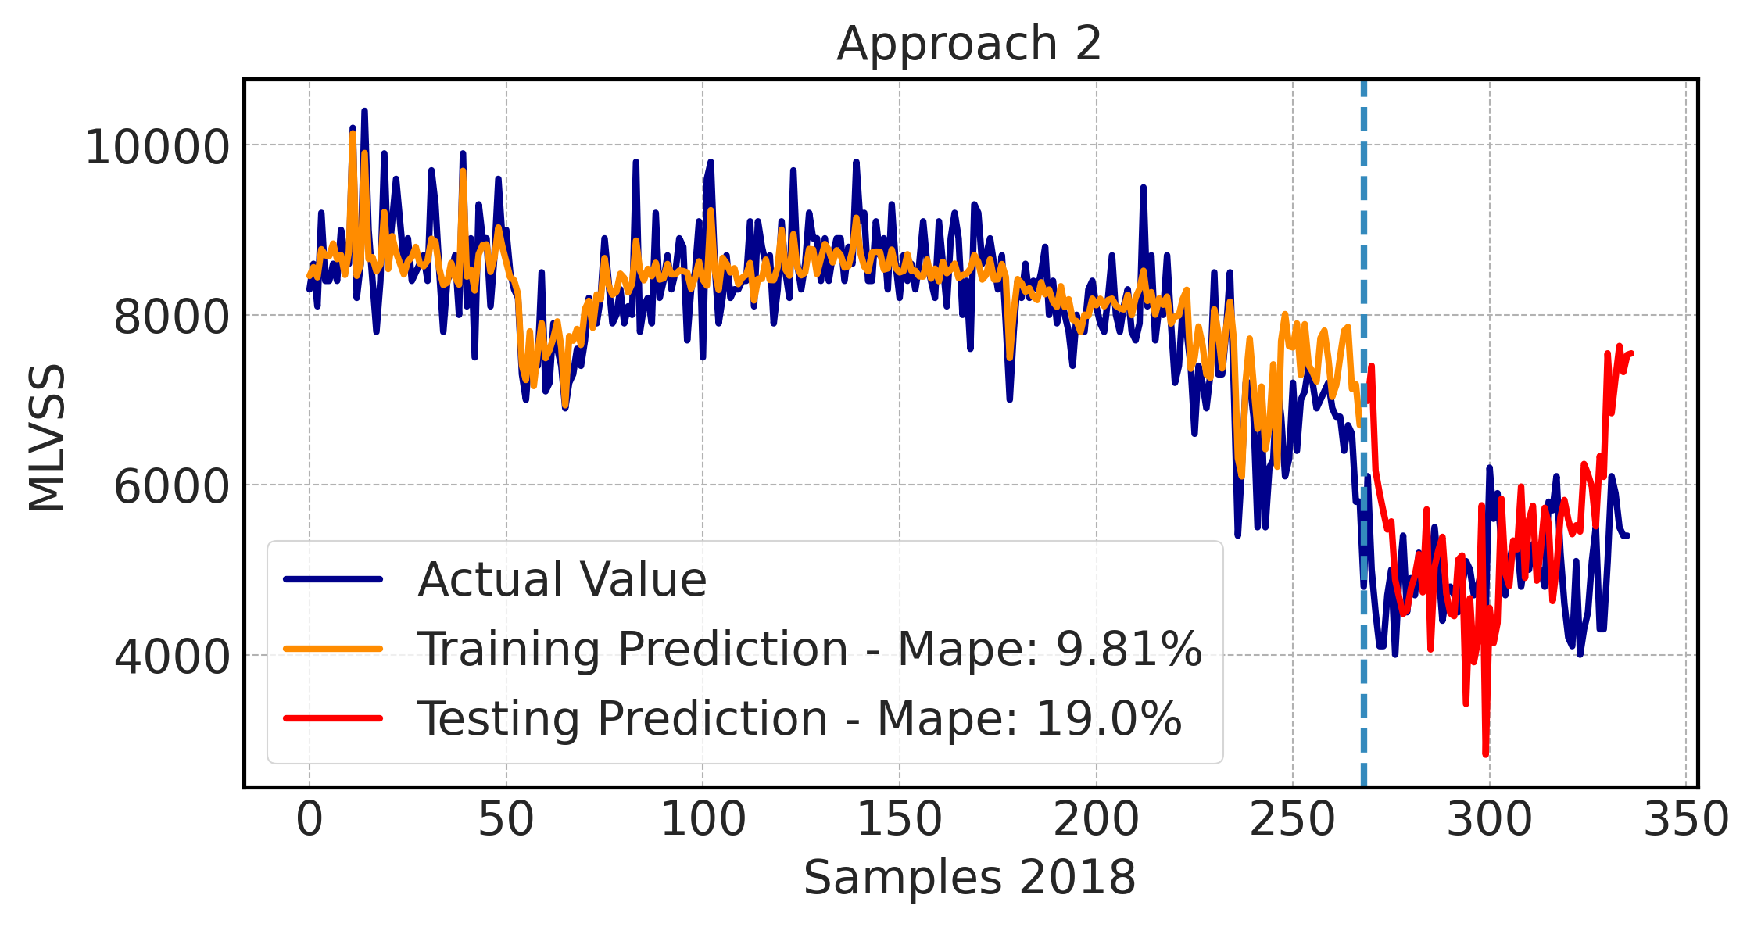
\includegraphics[width=\linewidth]{figures/Ch5/MLVSS-approach2.pdf}
\caption{Approach 2 - MLVSS}
\label{f:App2-MLVSS}
\end{figure}

\begin{itemize}
    \item Loss = mse
    \item Optimizer = Adam
    \item Activation =  Linear
    \item Number of Layers = 2
    \item Number of Neurons per layer = [4, 10]
    \item Batch Normalization = 1
    \item Dropout = 0
\end{itemize}

%-----------------------------------------------
\section{Approach 3}

\begin{figure}[h!]
\centering
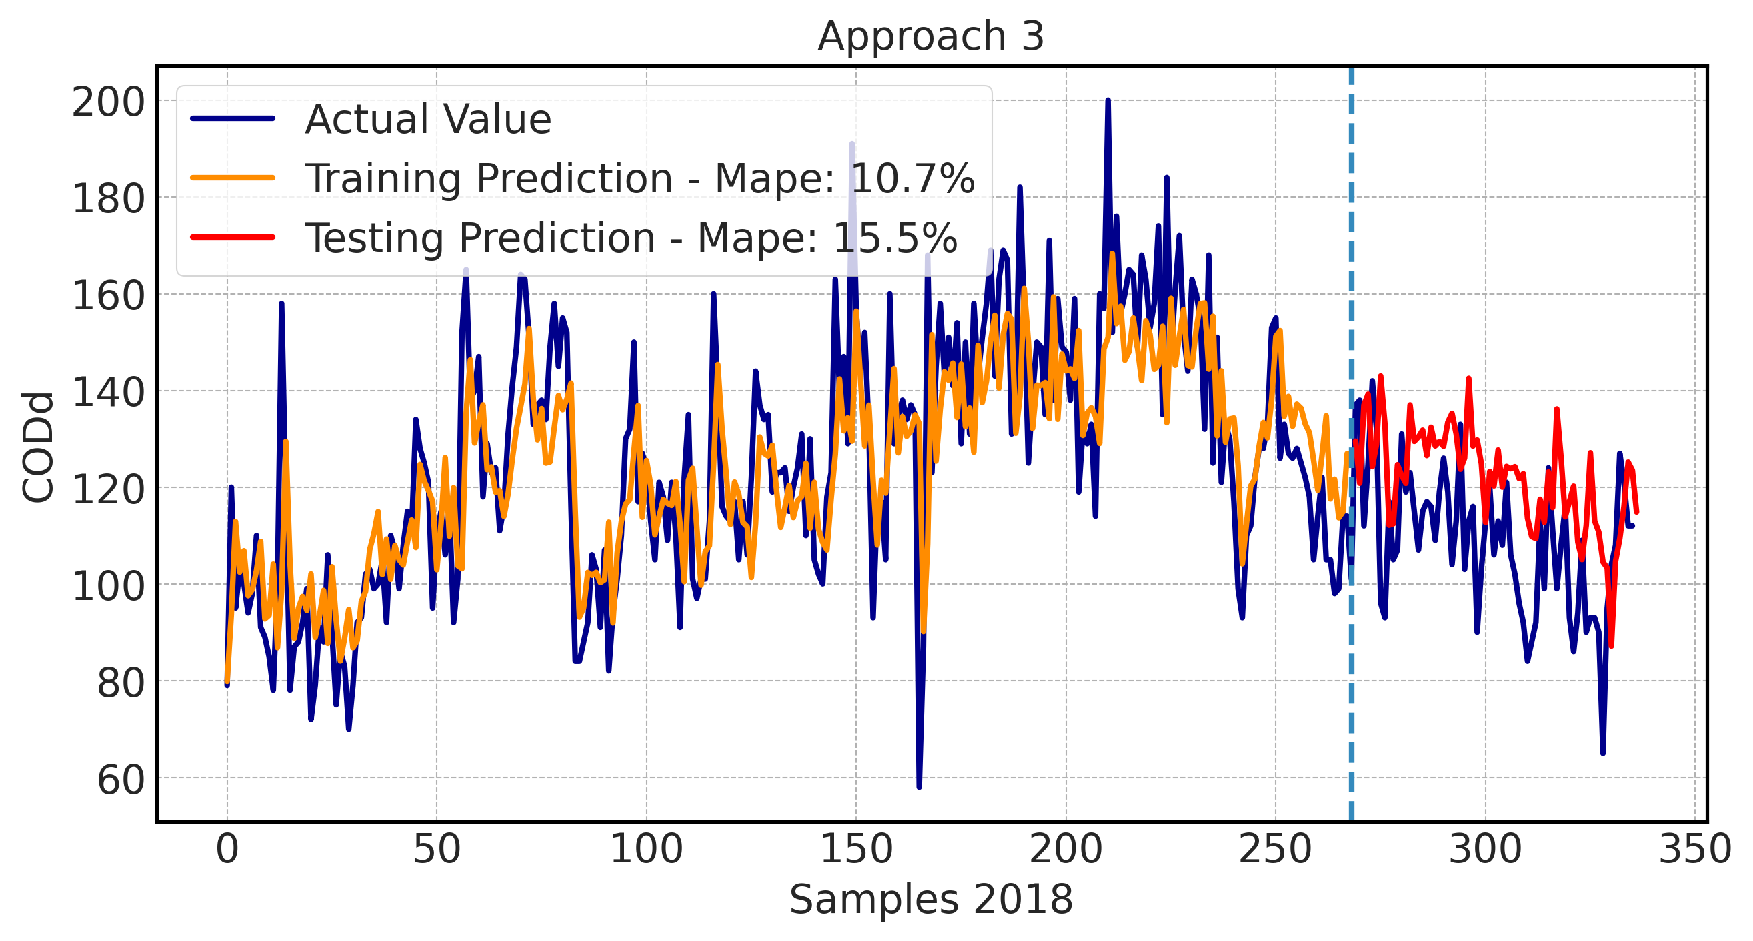
\includegraphics[width=\linewidth]{figures/Ch5/CODd-3.pdf}
\caption{Approach 3 - COD\textsubscript{D}}
\label{f:App3-codd}
\end{figure}

The last approach predicts using \ac{SVR} algorithm.

\begin{figure}[h!]
\centering
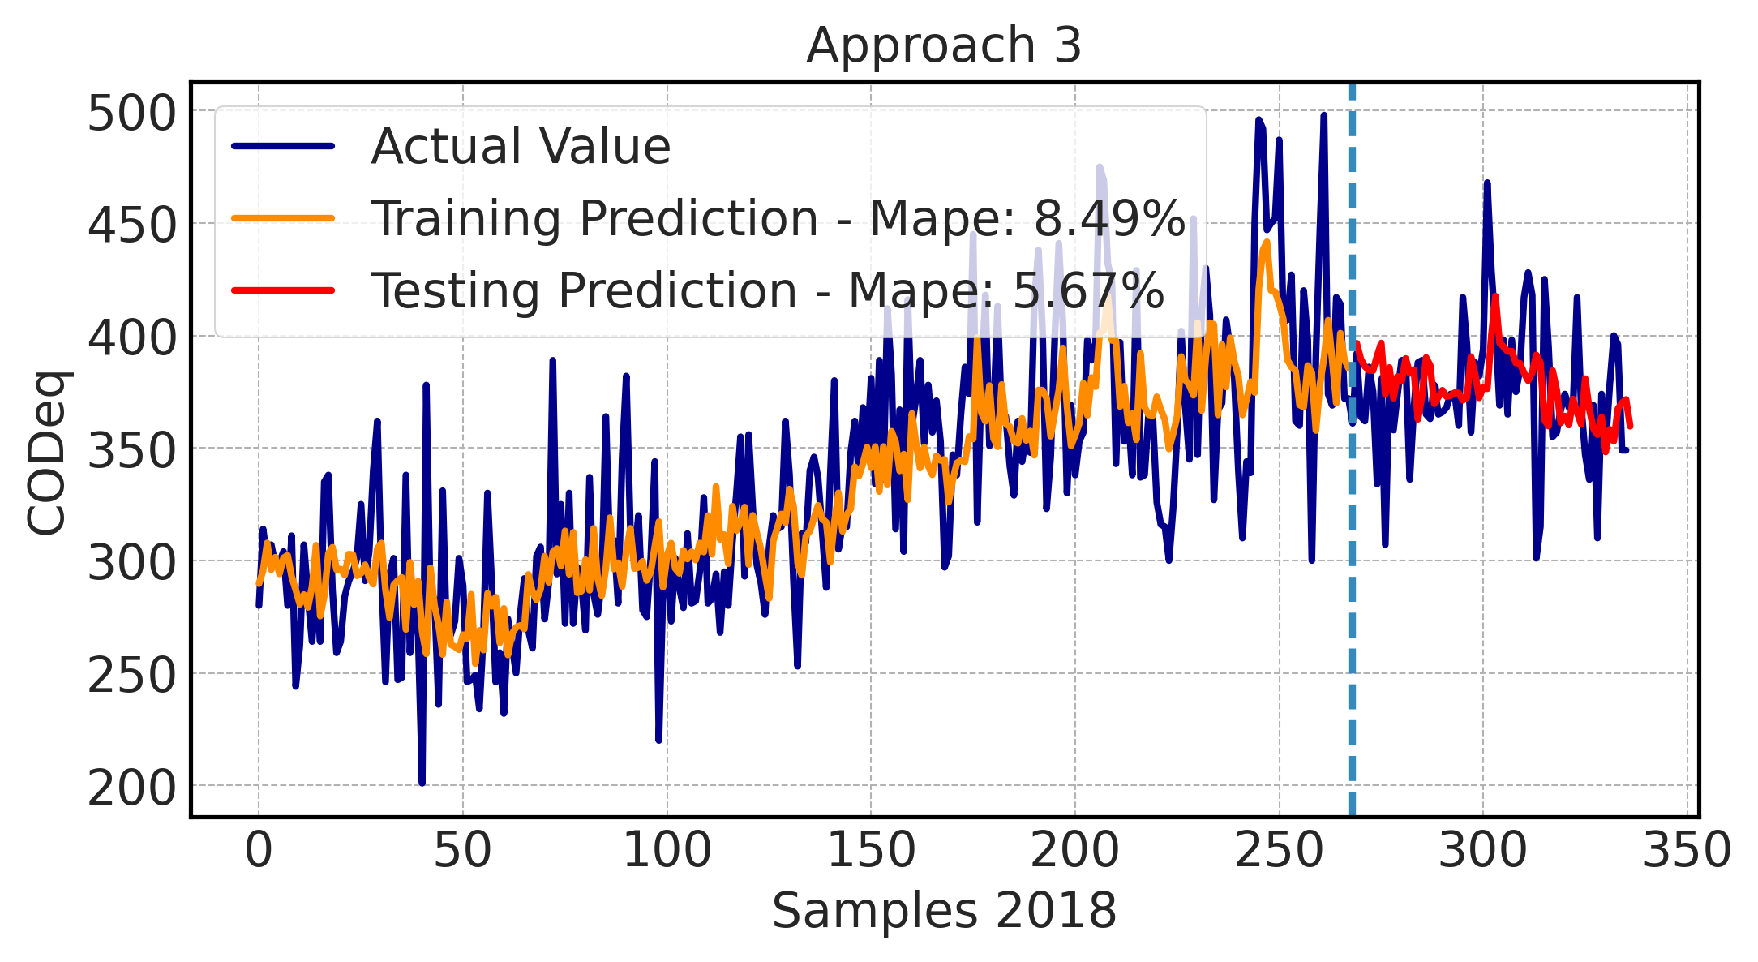
\includegraphics[width=\linewidth]{figures/Ch5/CODeq-3.pdf}
\caption{Approach 3 - COD\textsubscript{EQ}}
\label{f:App3-codeq}
\end{figure}

\begin{figure}[h!]
\centering
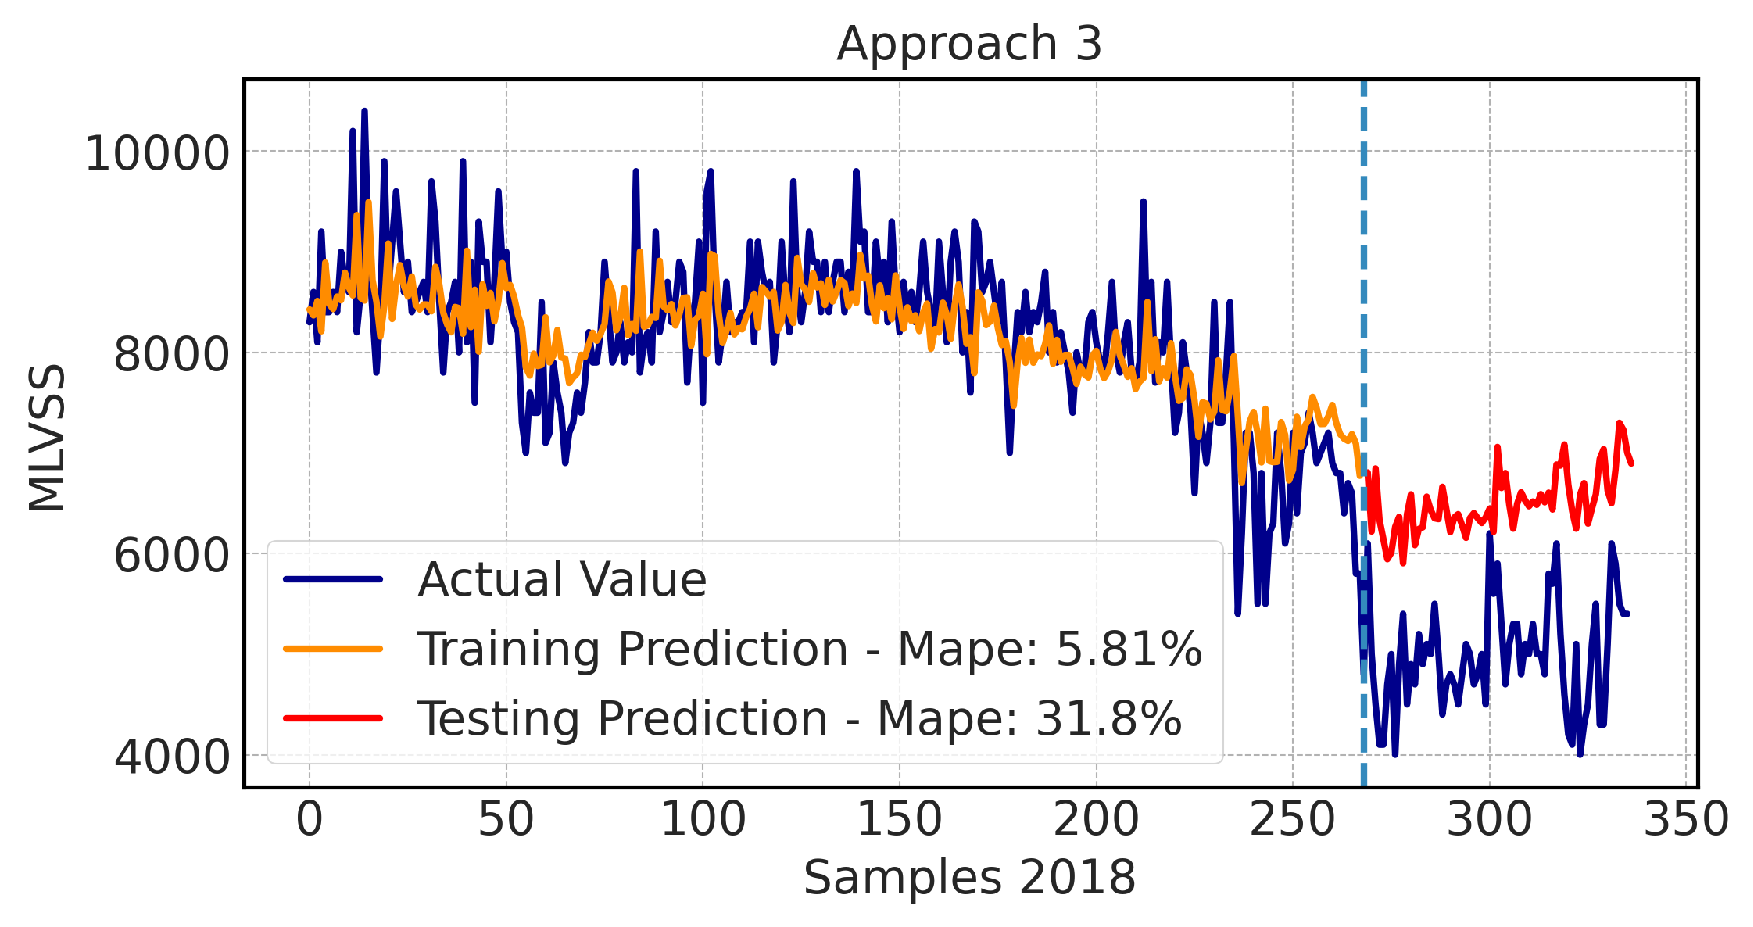
\includegraphics[width=\linewidth]{figures/Ch5/MLVSS-approach3.pdf}
\caption{Approach 3 - MLVSS}
\label{f:App3-MLVSS}
\end{figure}

This third model sometimes presents a shift prediction respect the expected value, nonetheless it achieves a good prediction. \autoref{f:App3-codd}, \autoref{f:App3-codeq}, and \autoref{f:App3-MLVSS} show the prediction results of this approach. 
\clearpage

%-----------------------------------------------
\section{Ensemble Approach 1 - Average}
The first ensemble approach makes an average of all three models presented before. \autoref{f:avg-codd}, \autoref{f:avg-codeq} and \autoref{f:avg-MLVSS} show the results of the average ensemble prediction for COD\textsubscript{D}, COD\textsubscript{EQ}, and MLVSS, respectively. 

\begin{figure}[h]
\centering
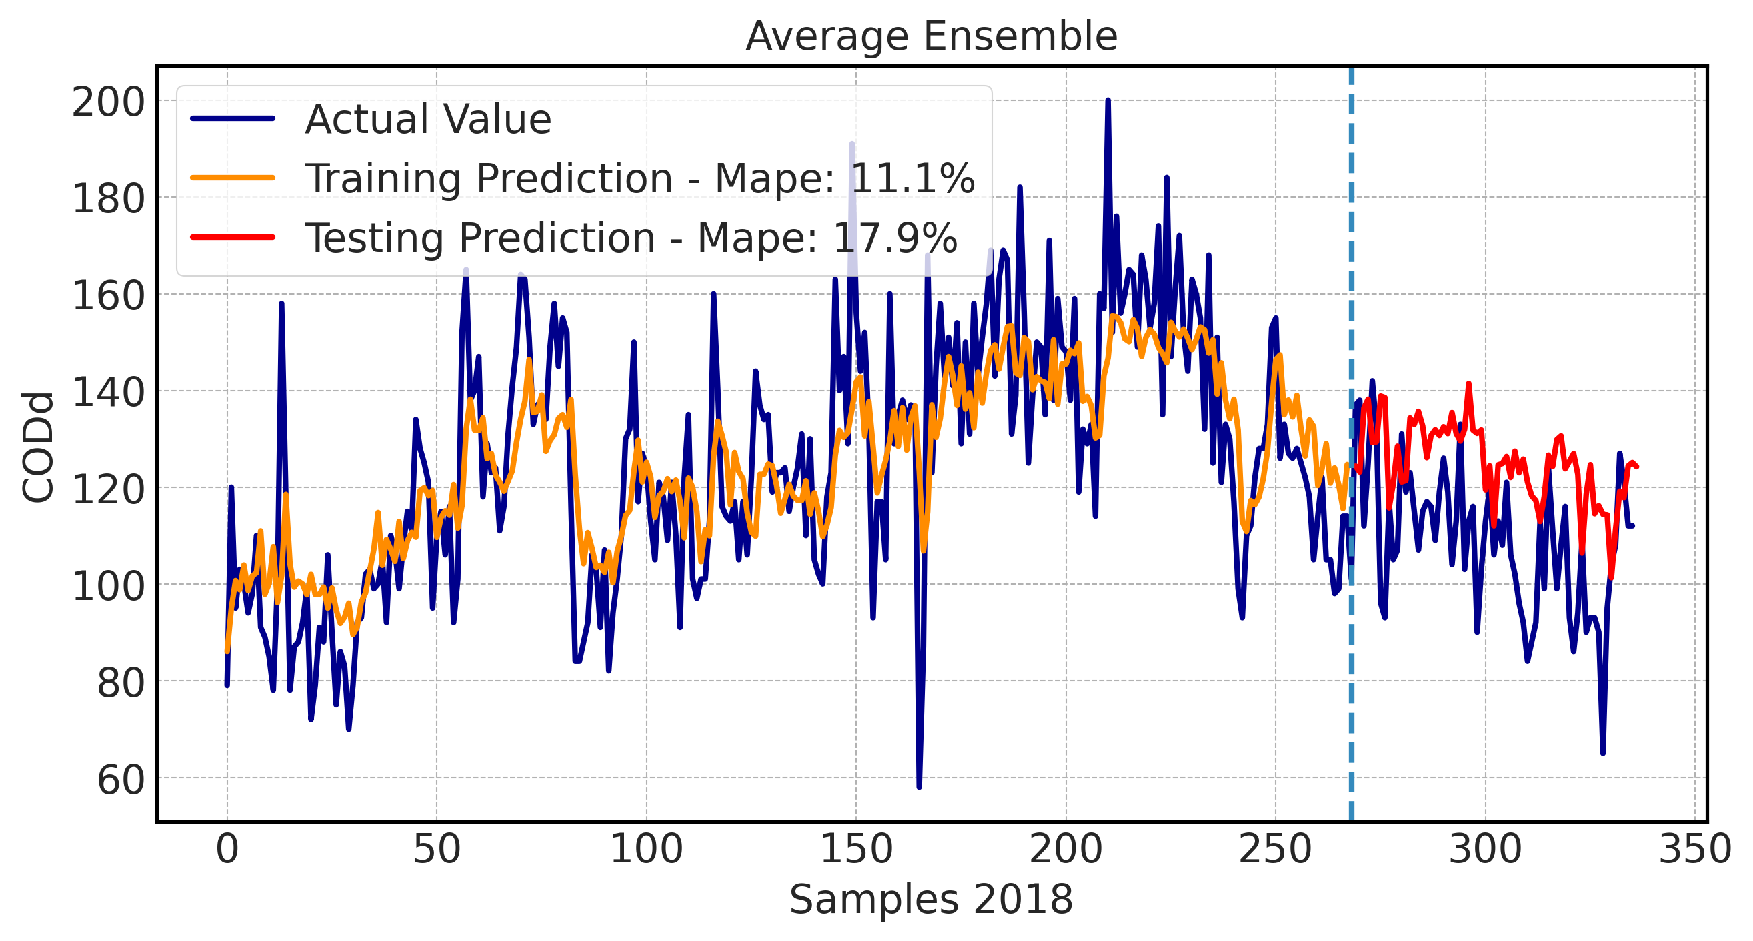
\includegraphics[width=\linewidth]{figures/Ch5/CODd-avg.pdf}
\caption{Average Ensemble - COD\textsubscript{D}}
\label{f:avg-codd}
\end{figure}

\begin{figure}[h]
\centering
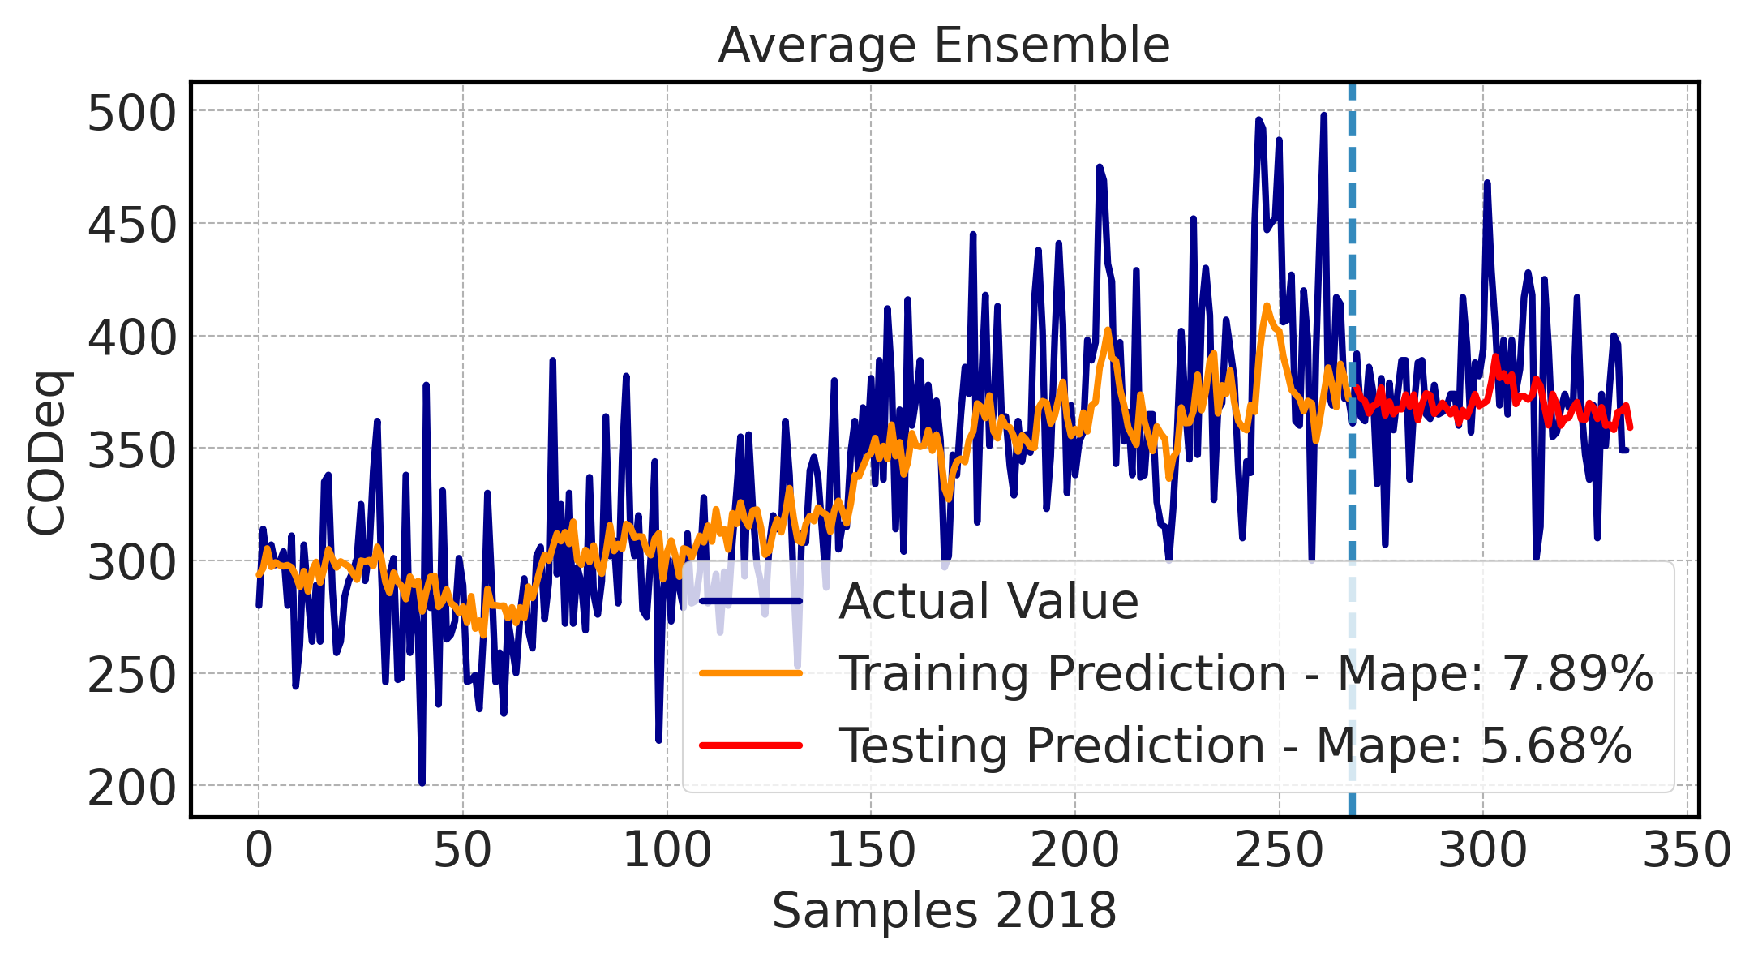
\includegraphics[width=\linewidth]{figures/Ch5/CODeq-avg.pdf}
\caption{Average Ensemble - COD\textsubscript{EQ}}
\label{f:avg-codeq}
\end{figure}

\begin{figure}[h]
\centering
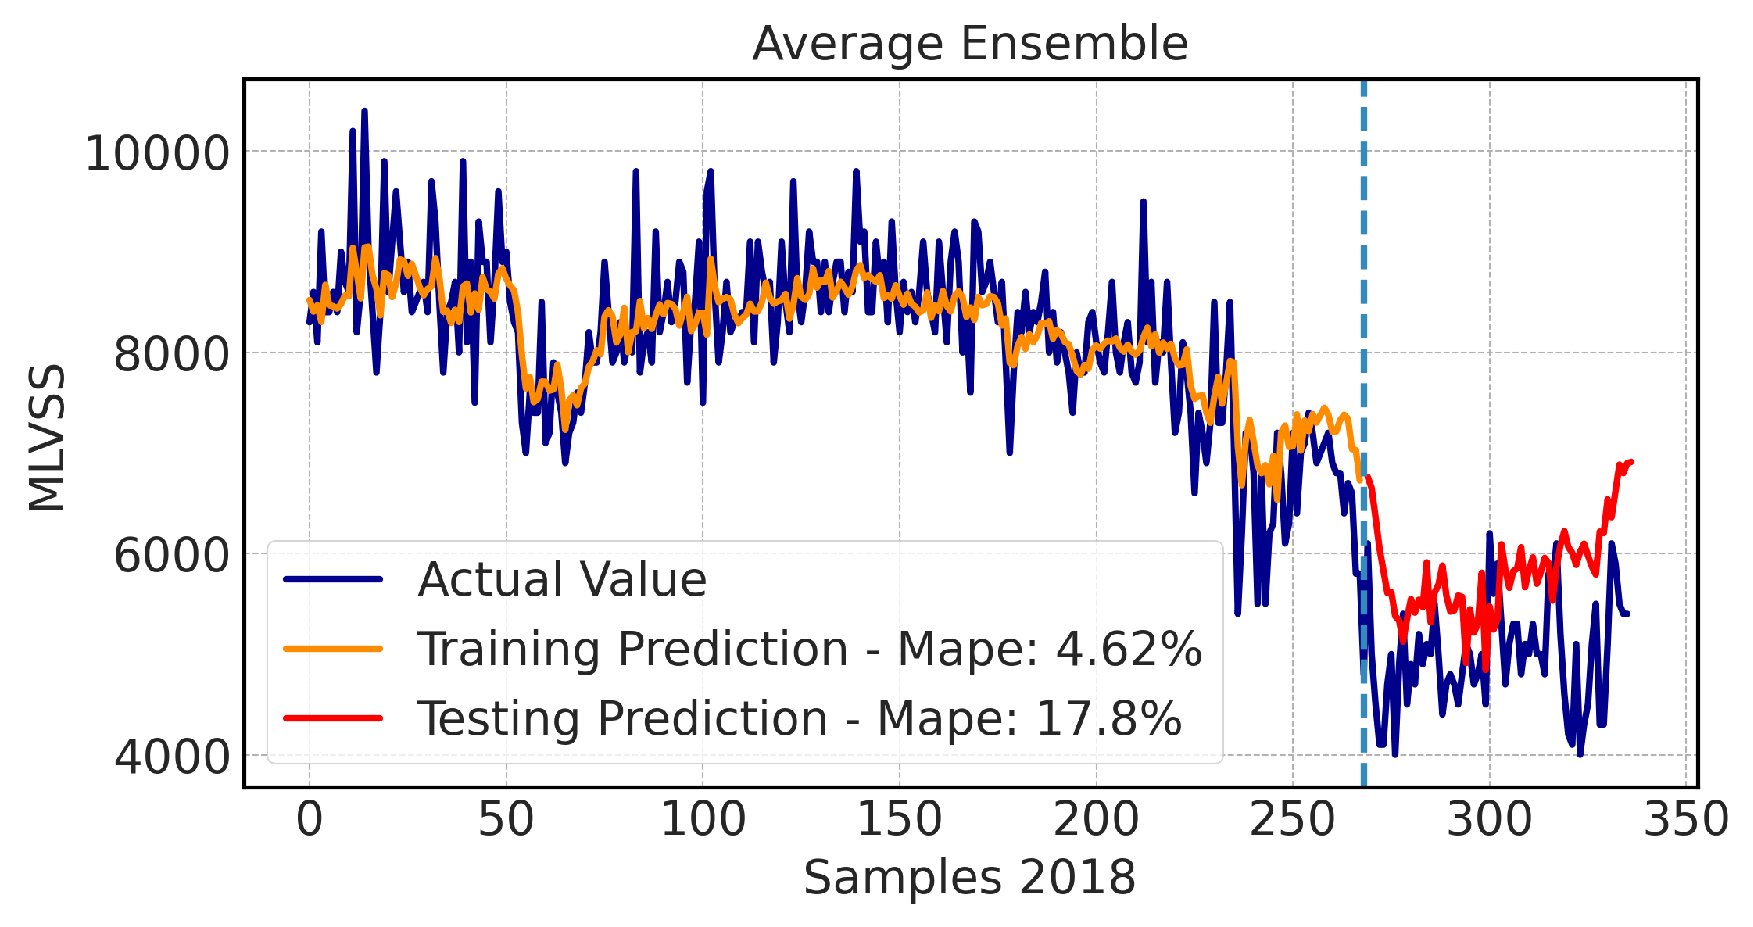
\includegraphics[width=\linewidth]{figures/Ch5/MVLSS-E_avg.pdf}
\caption{Average Ensemble - MLVSS}
\label{f:avg-MLVSS}
\end{figure}

%-----------------------------------------------
\section{Ensemble Approach 2 - MLP Fusion}
The second ensemble approach fuses all three models output presented before using a \ac{MLP}, and uses the exogenous variables as information source to enhance the final prediction. \autoref{f:avg-codd}, \autoref{f:avg-codeq} and \autoref{f:avg-MLVSS} show the results of the \ac{MLP} fusion ensemble prediction for the target variables. 

\begin{figure}[h]
\centering
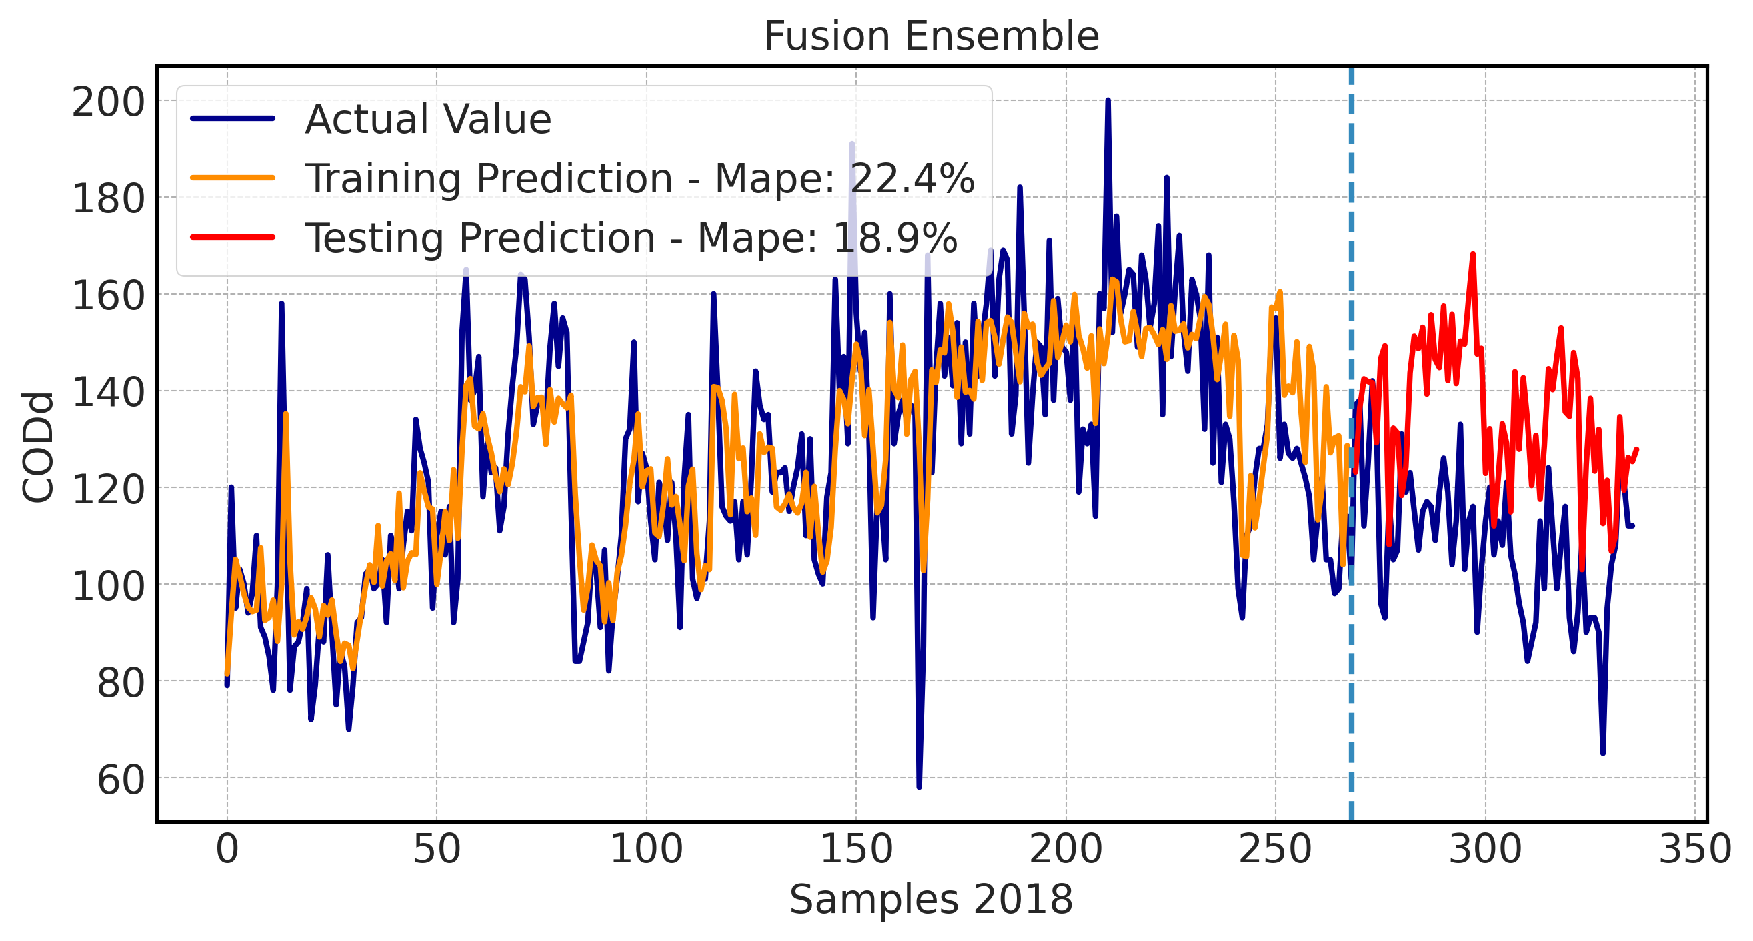
\includegraphics[width=\linewidth]{figures/Ch5/CODd-ann.pdf}
\caption{MLP Ensemble - COD\textsubscript{D}}
\label{f:ann-codd}
\end{figure}

\begin{figure}[h]
\centering
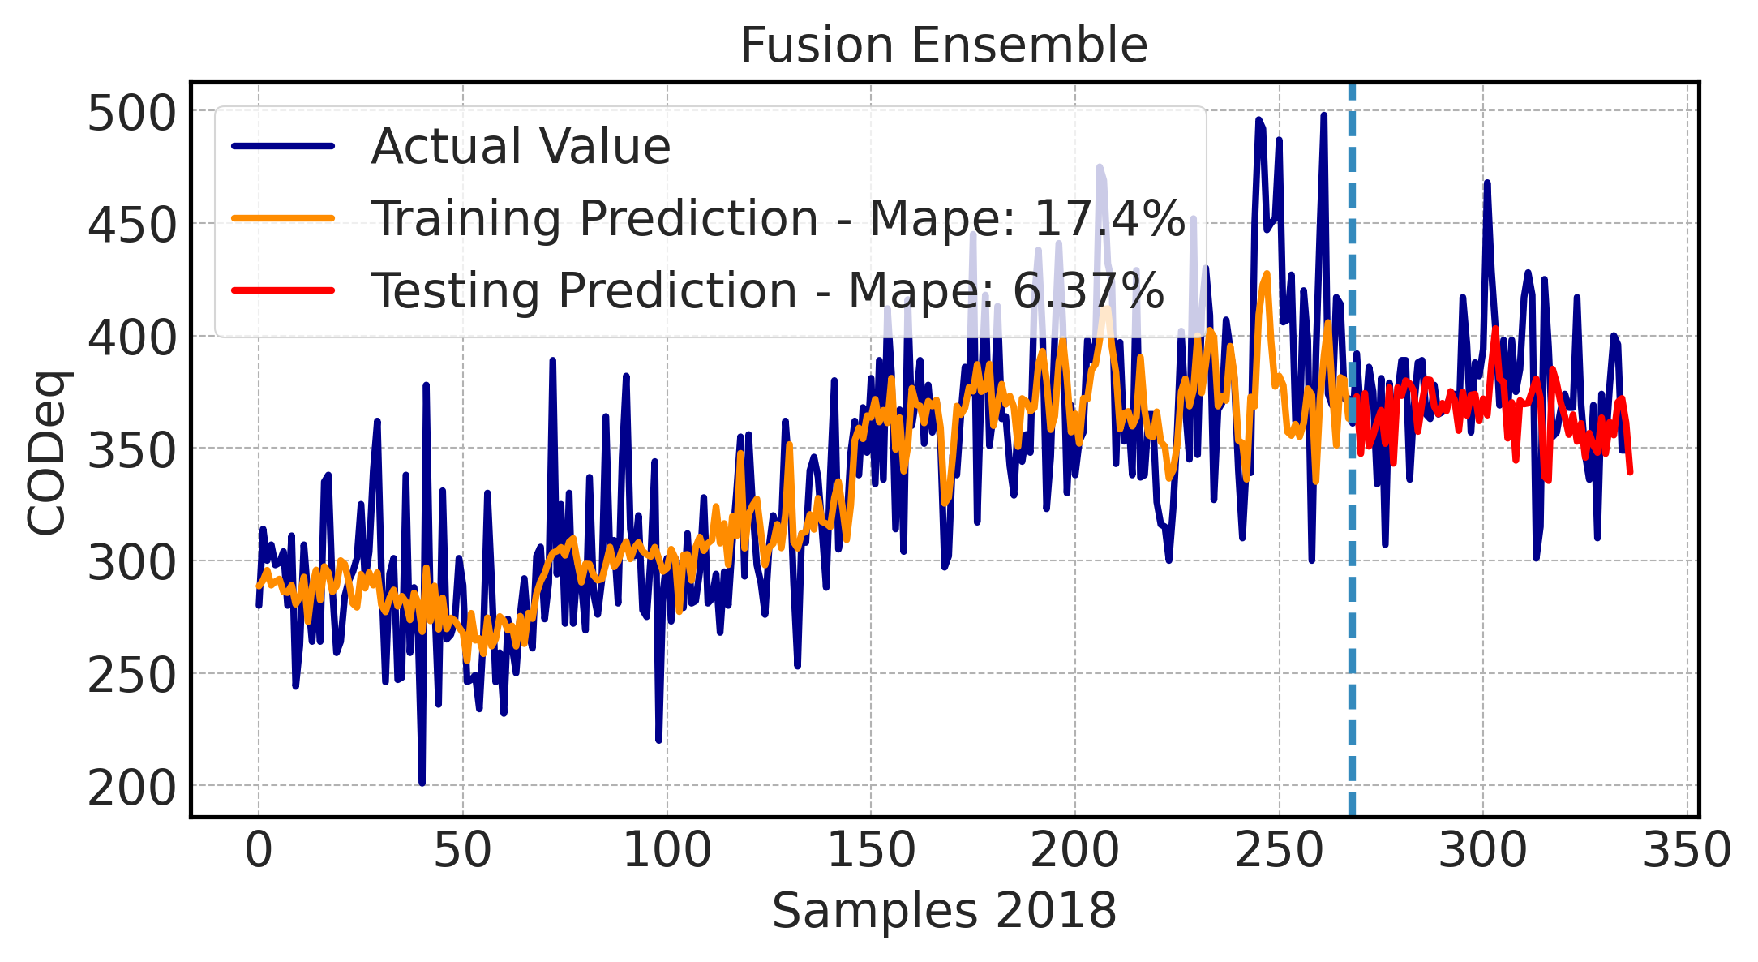
\includegraphics[width=\linewidth]{figures/Ch5/CODeq-ann.pdf}
\caption{MLP Ensemble - COD\textsubscript{EQ}}
\label{f:ann-codeq}
\end{figure}

\begin{figure}[h]
\centering
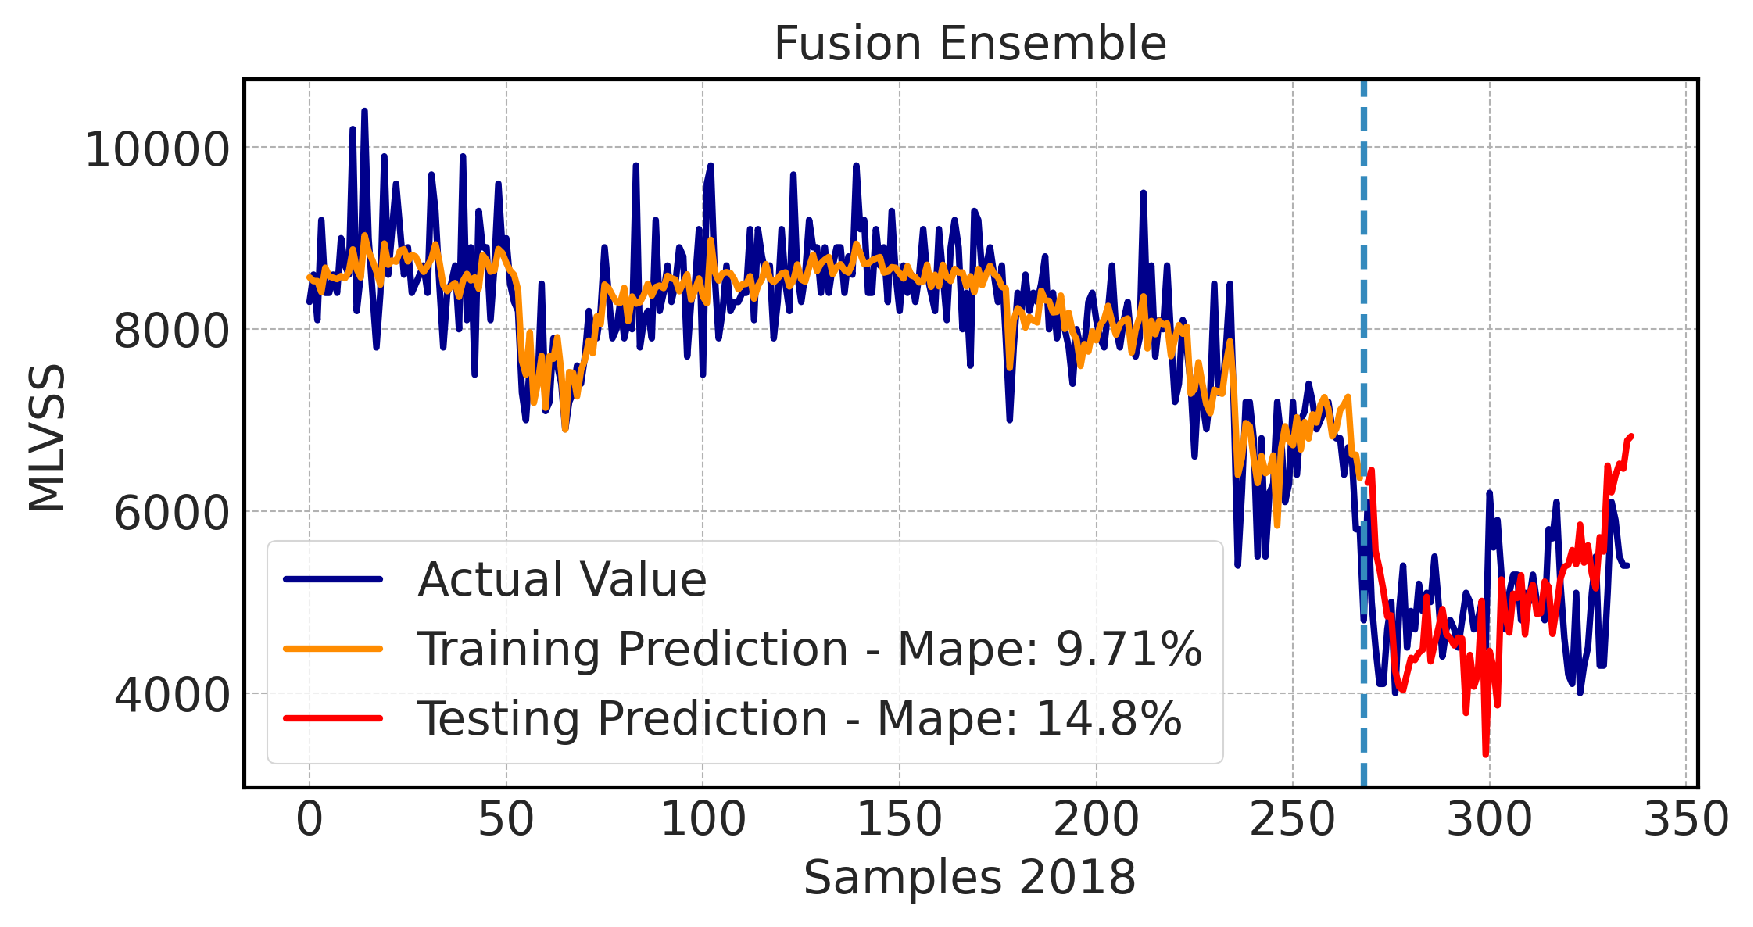
\includegraphics[width=\linewidth]{figures/Ch5/MVLSS-E_ann.pdf}
\caption{MLP Ensemble - MLVSS}
\label{f:ann-MLVSS}
\end{figure}

%-----------------------------------------------
\section{Ensemble Approach 3 - Selection}
The last ensemble approach predicts which model will perform best based on the process conditions represented by the exogenous variables. This prediction allows selecting one of the single models as the most suitable one to carry out the prediction. \autoref{f:avg-codd}, \autoref{f:avg-codeq} and \autoref{f:avg-MLVSS} show the results of this ensemble approach prediction for the target variables. 

\begin{figure}[h!]
\centering
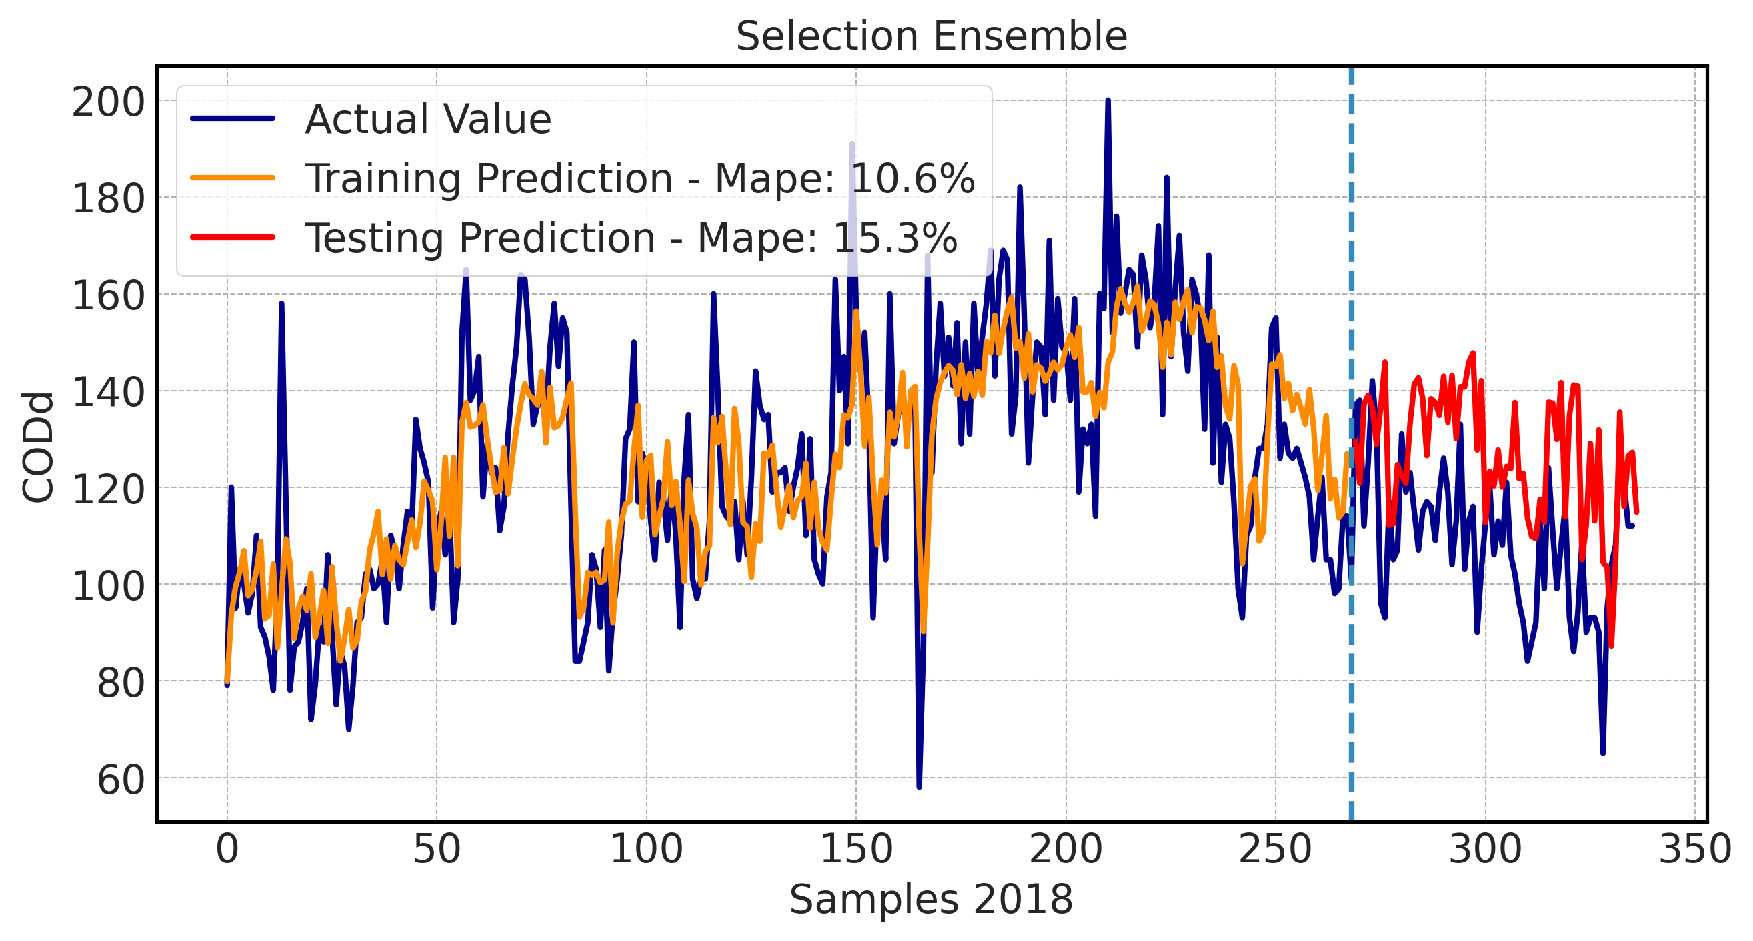
\includegraphics[width=\linewidth]{figures/Ch5/CODd-ann2.pdf}
\caption{MLP Ensemble - COD\textsubscript{D}}
\label{f:ann2-codd}
\end{figure}

\begin{figure}[h!]
\centering
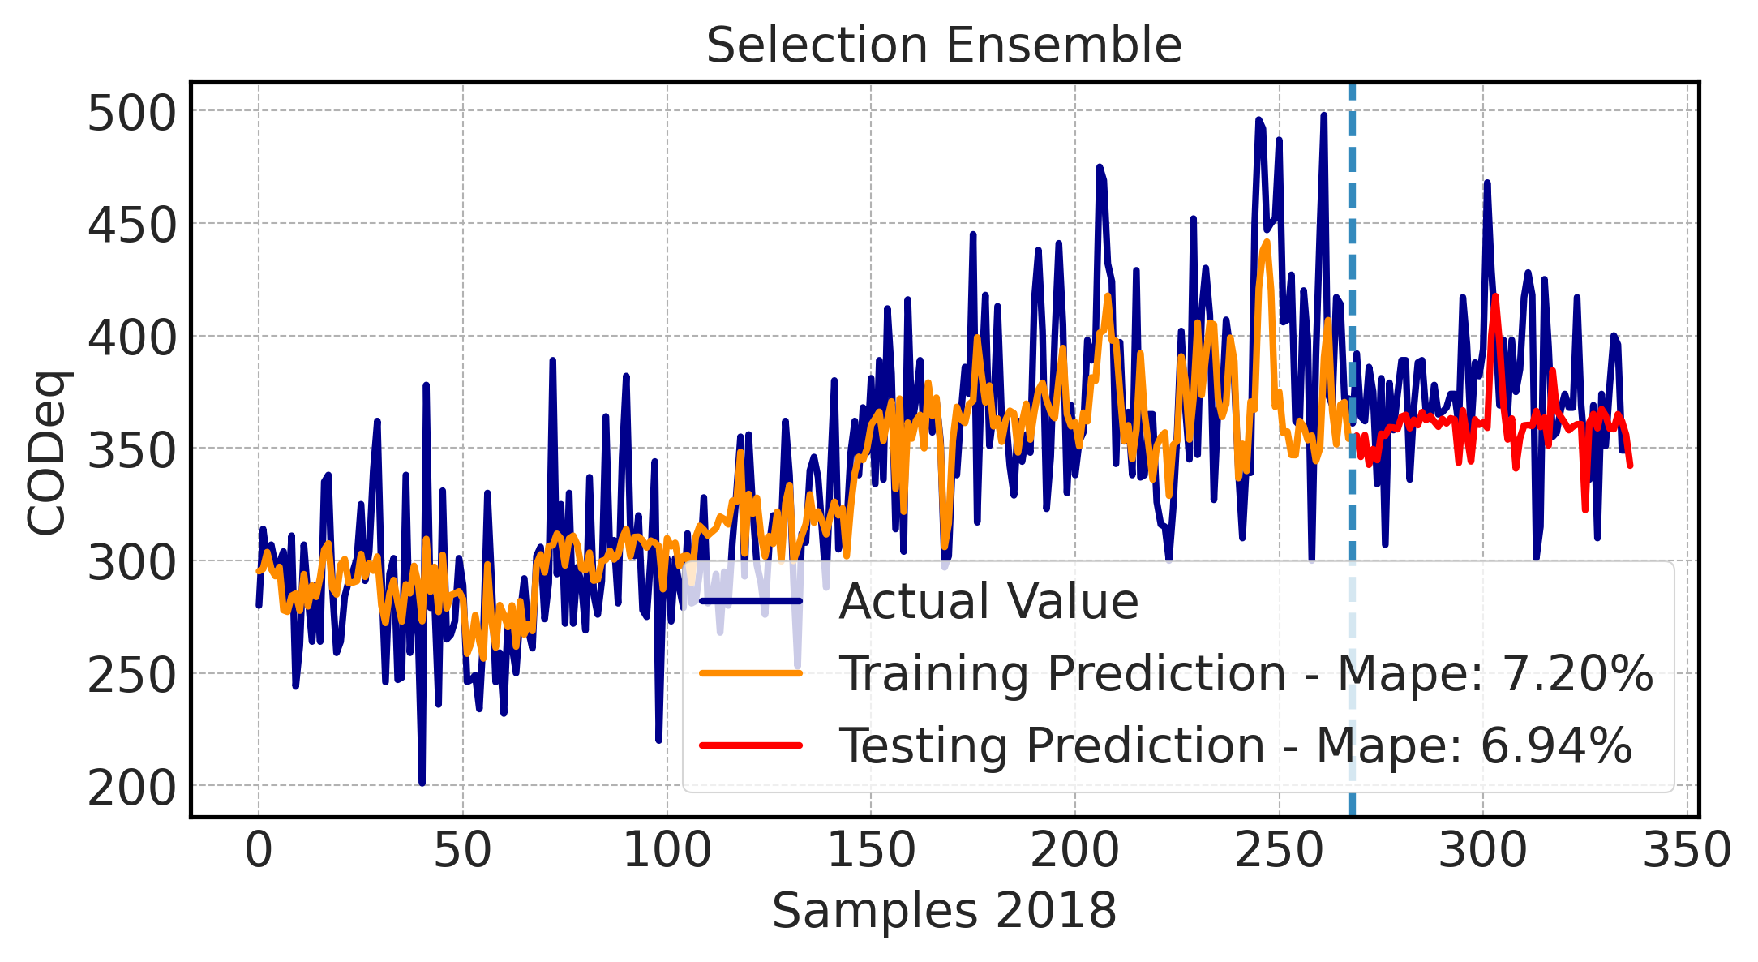
\includegraphics[width=\linewidth]{figures/Ch5/CODeq-ann2.pdf}
\caption{MLP Ensemble - COD\textsubscript{EQ}}
\label{f:ann2-codeq}
\end{figure}

\begin{figure}[h!]
\centering
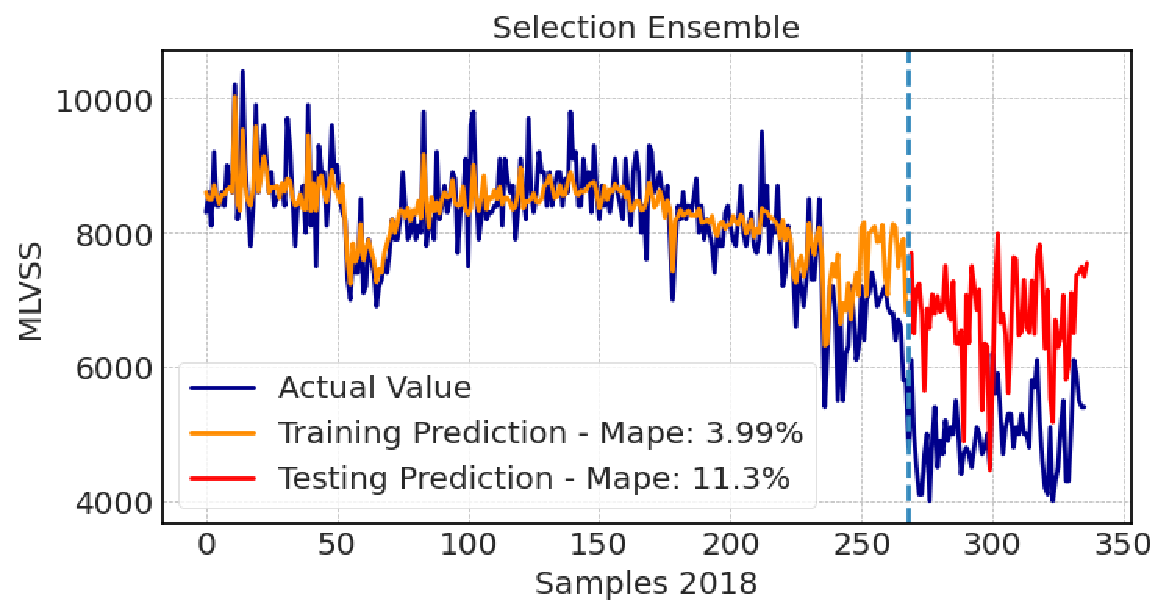
\includegraphics[width=\linewidth]{figures/Ch5/MVLSS-E_ann2.pdf}
\caption{MLP Ensemble - MLVSS}
\label{f:ann2-MLVSS}
\end{figure}

\section{Discussion}
\label{s:Contribution-2-Summary}

This chapter presents the implementation and obtained results of three approaches to predict time series variables of the wastewater treatment process. Also, three different ensemble approaches are presented to enhance the intelligent system prediction performance.
\autoref{t:Results} summarizes the \ac{MAPE} results obtained by the single models and the ensemble approaches. It is worth mentioning that hyper-parameters tuning was made using the training set as well as the evaluation of ensemble model enhancement. The best model performance over the training is highlighted in bold. The ensemble models offer a more robust prediction and present some improvements in \ac{MAPE}\%.
%\begin{longtable}{@{}l *{2}{rr}}
\begin{longtable}[h]{@{}l *{6}{rr}}
\caption[Approaches results]{Approaches results}
\label{t:Results}
\\
%   
\toprule%


 {\bfseries MAPE } & {\bfseries App.1} & ~ & {\bfseries App.2} & ~ & {\bfseries App.3} & ~ & {\bfseries Ens.1} & ~ & {\bfseries Ens.2} & ~ & {\bfseries Ens.3}
\\

\cmidrule[0.4pt](r{0.125em}){1-1}%
\cmidrule[0.4pt](lr{0.125em}){2-3}%
\cmidrule[0.4pt](lr{0.125em}){4-5}%
\cmidrule[0.4pt](lr{0.125em}){6-7}%
\cmidrule[0.4pt](lr{0.125em}){8-9}%
\cmidrule[0.4pt](lr{0.125em}){10-11}%
\cmidrule[0.4pt](lr{0.125em}){12-13}%


  \endfirsthead

\endhead


        (\%) & Train & Test & Train & Test & Train & Test & Train & Test & Train & Test & Train & Test  \\ 
        \hline
        MVLSS & 5.23 & 9.2 & 9.81 & 19.0 & 5.81 & 31.8 & 4.62 & 17.8 & 9.71 & 14.8 & \textbf{3.99} & 11.3  \\ 
        COD\textsubscript{EQ} & 8.6 & 6.21 & 16.1 & 7.59 & 8.49 & 5.67 & 7.89 & 5.68 & 17.4 & 6.37 & \textbf{7.2} & 6.94  \\ 
        COD\textsubscript{D} & 11.6 & 13.7 & 21.3 & 26.5 & 10.7 & 15.5 & 11.1 & 17.9 & 22.4 & 18.9 & \textbf{10.6} & 15.3  \\ 


\bottomrule

\end{longtable}
